\section{Results and Discussion}
\label{sec:results}
\begin{figure*}[t]
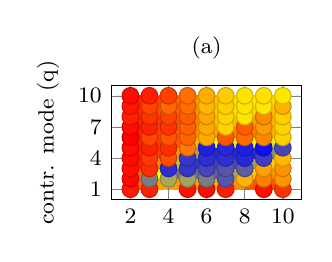
\begin{tikzpicture}
\begin{axis}
[
width=0.33\textwidth,
height=0.25\textwidth,
style={font=\footnotesize},
grid=major,
grid style={dotted},
align=center,
%xlabel={tensor order},
ylabel={contr. mode (q)},
title={{(a)}}, %  bgemm, asymmetric
scaled ticks=false,
zlabel={GFlops},
view={0}{90}, 
ytick={1,4,7,10},
xtick={2,4,6,8,10},
xmin=1, xmax=11,
ymin=0, ymax=11,
try min ticks=8,
zmin=300, zmax=2300,
point meta min=300, point meta max=2300,
colormap/hot, 
samples=50,
%colorbar sampled,
%colorbar/width=0.2cm,
%colorbar style={
%	point meta min=300, point meta max=2300,
%	samples=50,
%	font=\footnotesize,
%	ytick={300,1300,2300},
%	yticklabels={0.3,1.3,2.3},
%	%title={\scriptsize Gflops},
%	%ylabel={\scriptsize Gflops},
%}
]
%\addplot3[mesh, scatter,samples=50,shader=interp]
%\addplot3[only marks, mesh, scatter,scatter src=z,samples=50,] % z buffer=sort, scatter src=z,
\addplot3[contour filled={number=100},scatter,shader=flat,samples=50]
%\addplot3+[mesh,scatter,shader=flat corner,samples=50, only marks, mark size=2]
coordinates{
	
(2.000,1.000,2142.734) (2.000,2.000,2241.014) (2.000,3.000,2205.546) (2.000,4.000,2226.263) (2.000,5.000,2232.877) (2.000,6.000,2281.816) (2.000,7.000,2222.317) (2.000,8.000,2122.831) (2.000,9.000,2166.437) (2.000,10.000,2231.354) 

(3.000,1.000,2104.803) (3.000,2.000,620.292) (3.000,3.000,2053.810) (3.000,4.000,1989.460) (3.000,5.000,2100.108) (3.000,6.000,1923.866) (3.000,7.000,2109.798) (3.000,8.000,2032.918) (3.000,9.000,1931.835) (3.000,10.000,2137.550) 

(4.000,1.000,2303.560) (4.000,2.000,742.055) (4.000,3.000,436.752) (4.000,4.000,1889.266) (4.000,5.000,2050.848) (4.000,6.000,1845.429) (4.000,7.000,2029.757) (4.000,8.000,1947.246) (4.000,9.000,1753.968) (4.000,10.000,1945.836) 

(5.000,1.000,2197.949) (5.000,2.000,727.736) (5.000,3.000,441.734) (5.000,4.000,458.055) (5.000,5.000,1643.657) (5.000,6.000,1763.676) (5.000,7.000,1793.195) (5.000,8.000,1799.906) (5.000,9.000,1726.622) (5.000,10.000,1710.693) 

(6.000,1.000,2225.857) (6.000,2.000,621.489) (6.000,3.000,489.438) (6.000,4.000,435.500) (6.000,5.000,386.554) (6.000,6.000,1410.907) (6.000,7.000,1419.437) (6.000,8.000,1428.795) (6.000,9.000,1330.280) (6.000,10.000,1386.923) 

(7.000,1.000,2137.668) (7.000,2.000,530.662) (7.000,3.000,532.587) (7.000,4.000,439.307) (7.000,5.000,400.923) (7.000,6.000,1835.402) (7.000,7.000,1186.143) (7.000,8.000,1195.514) (7.000,9.000,1211.432) (7.000,10.000,1230.143) 

(8.000,1.000,2411.000) (8.000,2.000,1340.829) (8.000,3.000,546.729) (8.000,4.000,405.255) (8.000,5.000,381.061) (8.000,6.000,1724.053) (8.000,7.000,1816.684) (8.000,8.000,1103.276) (8.000,9.000,1109.365) (8.000,10.000,1119.582) 

(9.000,1.000,2215.896) (9.000,2.000,1637.409) (9.000,3.000,1448.314) (9.000,4.000,477.752) (9.000,5.000,353.959) (9.000,6.000,1596.361) (9.000,7.000,1496.308) (9.000,8.000,1566.431) (9.000,9.000,1085.107) (9.000,10.000,1135.908) 

(10.000,1.000,2011.147) (10.000,2.000,1504.412) (10.000,3.000,1538.421) (10.000,4.000,1335.732) (10.000,5.000,483.993) (10.000,6.000,1202.734) (10.000,7.000,1197.316) (10.000,8.000,1213.834) (10.000,9.000,1362.208) (10.000,10.000,1087.708)


};
\end{axis}
\end{tikzpicture}
\hfill
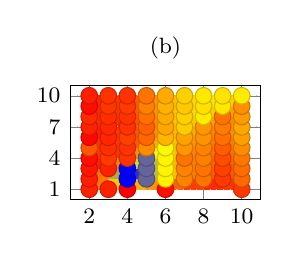
\begin{tikzpicture}
\begin{axis}
[
width=0.33\textwidth,
height=0.25\textwidth,
style={font=\footnotesize},
grid=major,
grid style={dotted},
align=center,
%xlabel={tensor order},
%ylabel={contr. mode (q)},
title={{(b)}}, %  ompfor<2d-slice> ttm<par-loops,seq-blas,$q$-slice>, asymmetric
scaled ticks=false,
zlabel={GFlops},
view={0}{90}, 
%view={-45}{45}, 
ytick={1,4,7,10},
xtick={2,4,6,8,10},
xmin=1, xmax=11,
ymin=0, ymax=11,
try min ticks=8,
zmin=300, zmax=2300,
point meta min=300, point meta max=2300,
colormap/hot, 
samples=50,
%colorbar sampled,
%colorbar/width=0.2cm,
%colorbar style={
%	point meta min=300, point meta max=2300,
%	samples=50,
%	font=\footnotesize,
%	ytick={300,1300,2300},
%	yticklabels={0.3,1.3,2.3},
%	%title={\scriptsize Gflops},
%	%ylabel={\scriptsize Gflops},
%}
]
%\addplot3[mesh, scatter,samples=50,shader=interp]
%\addplot3[only marks, mesh, scatter,scatter src=z,samples=50,] % z buffer=sort, scatter src=z,
\addplot3[contour filled={number=100},scatter,shader=flat,samples=50]
%\addplot3+[mesh,scatter,shader=flat corner,samples=50, only marks, mark size=2]
coordinates{

(2.000,1.000,2107.002) (2.000,2.000,2127.162) (2.000,3.000,2176.298) (2.000,4.000,2215.649) (2.000,5.000,1837.632) (2.000,6.000,2241.609) (2.000,7.000,2101.558) (2.000,8.000,2075.436) (2.000,9.000,2236.130) (2.000,10.000,2133.353) 

(3.000,1.000,2119.523) (3.000,2.000,167.437) (3.000,3.000,2112.420) (3.000,4.000,1989.285) (3.000,5.000,2041.921) (3.000,6.000,2084.201) (3.000,7.000,2080.454) (3.000,8.000,2046.614) (3.000,9.000,2013.009) (3.000,10.000,2024.421) 

(4.000,1.000,2285.299) (4.000,2.000,314.287) (4.000,3.000,311.849) (4.000,4.000,2011.869) (4.000,5.000,2039.029) (4.000,6.000,1944.642) (4.000,7.000,2023.178) (4.000,8.000,2033.385) (4.000,9.000,1992.379) (4.000,10.000,2039.303) 

(5.000,1.000,2475.804) (5.000,2.000,568.291) (5.000,3.000,562.230) (5.000,4.000,562.587) (5.000,5.000,1564.667) (5.000,6.000,1756.890) (5.000,7.000,1791.524) (5.000,8.000,1712.024) (5.000,9.000,1626.887) (5.000,10.000,1695.764) 

(6.000,1.000,2218.038) (6.000,2.000,1025.980) (6.000,3.000,1034.039) (6.000,4.000,1026.350) (6.000,5.000,945.367) (6.000,6.000,1340.191) (6.000,7.000,1422.937) (6.000,8.000,1402.244) (6.000,9.000,1375.707) (6.000,10.000,1411.432) 

(7.000,1.000,2307.246) (7.000,2.000,1602.074) (7.000,3.000,1617.348) (7.000,4.000,1682.539) (7.000,5.000,1516.443) (7.000,6.000,1446.511) (7.000,7.000,1229.353) (7.000,8.000,1202.606) (7.000,9.000,1245.855) (7.000,10.000,1211.880) 

(8.000,1.000,2441.539) (8.000,2.000,1699.771) (8.000,3.000,1686.405) (8.000,4.000,1622.372) (8.000,5.000,1600.438) (8.000,6.000,1530.707) (8.000,7.000,1508.466) (8.000,8.000,1073.808) (8.000,9.000,1123.363) (8.000,10.000,1096.486) 

(9.000,1.000,2330.060) (9.000,2.000,1985.056) (9.000,3.000,1941.312) (9.000,4.000,1892.533) (9.000,5.000,1805.699) (9.000,6.000,1706.515) (9.000,7.000,1658.818) (9.000,8.000,1693.350) (9.000,9.000,1093.684) (9.000,10.000,1112.530) 

(10.000,1.000,1988.818) (10.000,2.000,1750.516) (10.000,3.000,1728.226) (10.000,4.000,1678.568) (10.000,5.000,1576.395) (10.000,6.000,1476.492) (10.000,7.000,1429.733) (10.000,8.000,1496.574) (10.000,9.000,1557.162) (10.000,10.000,1068.719) 


};
\end{axis}
\end{tikzpicture}
\hfill
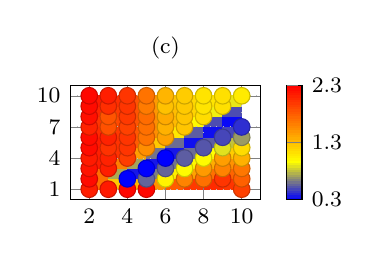
\begin{tikzpicture}
\begin{axis}
[
width=0.33\textwidth,
height=0.25\textwidth,
style={font=\footnotesize},
grid=major,
grid style={dotted},
align=center,
%xlabel={tensor order},
%ylabel={contr. mode (q)},
title={{(c)}}, %  ompfor<qd-slice> ttm<par-loops,seq-blas,$q$-slice>, asymmetric
scaled ticks=false,
zlabel={GFlops},
view={0}{90}, 
%view={-45}{45}, 
ytick={1,4,7,10},
xtick={2,4,6,8,10},
%xmin=2, xmax=10,
%ymin=1, ymax=10,
xmin=1, xmax=11,
ymin=0, ymax=11,
try min ticks=8,
zmin=300, zmax=2300,
point meta min=300, point meta max=2300,
%colormap/jet, 
colormap/hot, 
%colormap/blackwhite,
%colormap={whiteblack}{indices of colormap={\pgfplotscolormaplastindexof{blackwhite},...,0 of blackwhite}},
samples=50,
%colormap access=piecewise const,
colorbar sampled,
colorbar/width=0.2cm,
colorbar style={
	point meta min=300, point meta max=2300,
	samples=50,
	font=\footnotesize,
	ytick={300,1300,2300},
	yticklabels={0.3,1.3,2.3},
	%title={\scriptsize Gflops},
	%ylabel={\scriptsize Gflops},
}
]
%\addplot3[mesh, scatter,samples=50,shader=interp]
%\addplot3[only marks, mesh, scatter,scatter src=z,samples=50,] % z buffer=sort, scatter src=z,
\addplot3[contour filled={number=100},scatter,shader=flat,samples=50]
%\addplot3+[mesh,scatter,shader=flat corner,samples=50, only marks, mark size=2]
coordinates{

(2.000,1.000,2134.021) (2.000,2.000,2224.864) (2.000,3.000,2184.477) (2.000,4.000,2142.541) (2.000,5.000,2229.439) (2.000,6.000,2238.772) (2.000,7.000,2105.091) (2.000,8.000,2201.214) (2.000,9.000,2232.448) (2.000,10.000,2240.926) 

(3.000,1.000,2146.896) (3.000,2.000,167.544) (3.000,3.000,2121.476) (3.000,4.000,2105.304) (3.000,5.000,2027.717) (3.000,6.000,2104.722) (3.000,7.000,1866.561) (3.000,8.000,1855.180) (3.000,9.000,2041.894) (3.000,10.000,2122.692) 

(4.000,1.000,2244.985) (4.000,2.000,313.766) (4.000,3.000,167.879) (4.000,4.000,1973.457) (4.000,5.000,2013.391) (4.000,6.000,2010.678) (4.000,7.000,1949.136) (4.000,8.000,1989.844) (4.000,9.000,2017.192) (4.000,10.000,2015.899) 

(5.000,1.000,2250.694) (5.000,2.000,574.277) (5.000,3.000,315.908) (5.000,4.000,166.343) (5.000,5.000,1559.782) (5.000,6.000,1688.138) (5.000,7.000,1711.412) (5.000,8.000,1721.389) (5.000,9.000,1653.587) (5.000,10.000,1691.902) 

(6.000,1.000,2403.465) (6.000,2.000,1026.371) (6.000,3.000,576.699) (6.000,4.000,312.020) (6.000,5.000,160.917) (6.000,6.000,1443.174) (6.000,7.000,1370.699) (6.000,8.000,1414.204) (6.000,9.000,1283.900) (6.000,10.000,1351.446) 

(7.000,1.000,2305.894) (7.000,2.000,1613.830) (7.000,3.000,988.435) (7.000,4.000,554.792) (7.000,5.000,290.305) (7.000,6.000,157.356) (7.000,7.000,1270.432) (7.000,8.000,1266.914) (7.000,9.000,1255.620) (7.000,10.000,1224.914) 

(8.000,1.000,2437.239) (8.000,2.000,1706.219) (8.000,3.000,1489.110) (8.000,4.000,999.755) (8.000,5.000,531.137) (8.000,6.000,280.182) (8.000,7.000,148.892) (8.000,8.000,1156.621) (8.000,9.000,1110.478) (8.000,10.000,1116.944) 

(9.000,1.000,2355.395) (9.000,2.000,2003.839) (9.000,3.000,1603.752) (9.000,4.000,1477.309) (9.000,5.000,887.839) (9.000,6.000,492.554) (9.000,7.000,262.294) (9.000,8.000,150.408) (9.000,9.000,1129.997) (9.000,10.000,1121.143) 

(10.000,1.000,1944.959) (10.000,2.000,1789.054) (10.000,3.000,1665.441) (10.000,4.000,1375.291) (10.000,5.000,1147.731) (10.000,6.000,715.205) (10.000,7.000,422.658) (10.000,8.000,236.076) (10.000,9.000,136.520) (10.000,10.000,1078.495) 


};
\end{axis}
\end{tikzpicture}


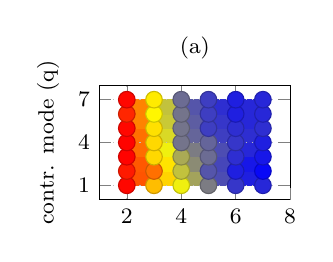
\begin{tikzpicture}
\begin{axis}
[
width=0.33\textwidth,
height=0.25\textwidth,
style={font=\footnotesize},
grid=major,
grid style={dotted},
align=center,
%xlabel={tensor order},
ylabel={contr. mode (q)},
title={{(a)}}, %  bgemm, asymmetric
scaled ticks=false,
zlabel={GFlops},
view={0}{90}, 
ytick={1,4,7,10},
xtick={2,4,6,8},
xmin=1, xmax=8,
ymin=0, ymax=8,
try min ticks=8,
zmin=0, zmax=2600,
point meta min=0, point meta max=2600,
colormap/hot, 
samples=50,
%colorbar sampled,
%colorbar/width=0.2cm,
%colorbar style={
%	point meta min=300, point meta max=2300,
%	samples=50,
%	font=\footnotesize,
%	ytick={300,1300,2300},
%	yticklabels={0.3,1.3,2.3},
%	%title={\scriptsize Gflops},
%	%ylabel={\scriptsize Gflops},
%}
]
%\addplot3[mesh, scatter,samples=50,shader=interp]
%\addplot3[only marks, mesh, scatter,scatter src=z,samples=50,] % z buffer=sort, scatter src=z,
\addplot3[contour filled={number=100},scatter,shader=flat,samples=50]
%\addplot3+[mesh,scatter,shader=flat corner,samples=50, only marks, mark size=2]
coordinates{

(2.000,1.000,2527.923) (2.000,2.000,2398.051) (2.000,3.000,2573.521) (2.000,4.000,2570.296) (2.000,5.000,2540.651) (2.000,6.000,2326.903) (2.000,7.000,2545.629) 

(3.000,1.000,1312.517) (3.000,2.000,1835.211) (3.000,3.000,1133.124) (3.000,4.000,1120.384) (3.000,5.000,1066.704) (3.000,6.000,915.932) (3.000,7.000,997.168) 

(4.000,1.000,825.045) (4.000,2.000,655.270) (4.000,3.000,579.750) (4.000,4.000,390.794) (4.000,5.000,411.134) (4.000,6.000,409.619) (4.000,7.000,375.457) 

(5.000,1.000,420.343) (5.000,2.000,308.678) (5.000,3.000,377.118) (5.000,4.000,348.232) (5.000,5.000,216.877) (5.000,6.000,232.073) (5.000,7.000,218.457) 

(6.000,1.000,206.774) (6.000,2.000,119.299) (6.000,3.000,167.691) (6.000,4.000,183.571) (6.000,5.000,179.989) (6.000,6.000,126.876) (6.000,7.000,128.135) 

(7.000,1.000,150.823) (7.000,2.000,33.170) (7.000,3.000,83.979) (7.000,4.000,128.221) (7.000,5.000,157.368) (7.000,6.000,143.557) (7.000,7.000,133.647) 


};
\end{axis}
\end{tikzpicture}
\hfill
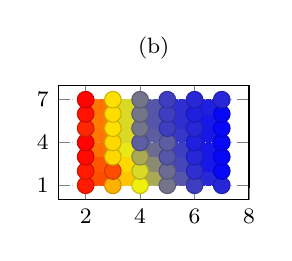
\begin{tikzpicture}
\begin{axis}
[
width=0.33\textwidth,
height=0.25\textwidth,
style={font=\footnotesize},
grid=major,
grid style={dotted},
align=center,
%xlabel={tensor order},
%ylabel={contr. mode (q)},
title={{(b)}}, %  ompfor<2d-slice> ttm<par-loops,seq-blas,$q$-slice>, asymmetric
scaled ticks=false,
zlabel={GFlops},
view={0}{90}, 
%view={-45}{45}, 
ytick={1,4,7,10},
xtick={2,4,6,8},
xmin=1, xmax=8,
ymin=0, ymax=8,
try min ticks=8,
zmin=0, zmax=2600,
point meta min=0, point meta max=2600,
colormap/hot, 
samples=50,
%colorbar sampled,
%colorbar/width=0.2cm,
%colorbar style={
%	point meta min=300, point meta max=2300,
%	samples=50,
%	font=\footnotesize,
%	ytick={300,1300,2300},
%	yticklabels={0.3,1.3,2.3},
%	%title={\scriptsize Gflops},
%	%ylabel={\scriptsize Gflops},
%}
]
%\addplot3[mesh, scatter,samples=50,shader=interp]
%\addplot3[only marks, mesh, scatter,scatter src=z,samples=50,] % z buffer=sort, scatter src=z,
\addplot3[contour filled={number=100},scatter,shader=flat,samples=50]
%\addplot3+[mesh,scatter,shader=flat corner,samples=50, only marks, mark size=2]
coordinates{

(2.000,1.000,2394.429) (2.000,2.000,2411.386) (2.000,3.000,2508.441) (2.000,4.000,2549.390) (2.000,5.000,2334.831) (2.000,6.000,2454.725) (2.000,7.000,2556.685) 

(3.000,1.000,1395.054) (3.000,2.000,2055.946) (3.000,3.000,1121.102) (3.000,4.000,1120.659) (3.000,5.000,1089.377) (3.000,6.000,1102.959) (3.000,7.000,1078.957) 

(4.000,1.000,819.991) (4.000,2.000,729.342) (4.000,3.000,579.869) (4.000,4.000,334.133) (4.000,5.000,390.153) (4.000,6.000,407.045) (4.000,7.000,394.057) 

(5.000,1.000,414.803) (5.000,2.000,369.532) (5.000,3.000,295.077) (5.000,4.000,318.473) (5.000,5.000,209.139) (5.000,6.000,214.825) (5.000,7.000,223.888) 

(6.000,1.000,208.097) (6.000,2.000,156.950) (6.000,3.000,141.868) (6.000,4.000,119.992) (6.000,5.000,134.757) (6.000,6.000,126.271) (6.000,7.000,133.034) 

(7.000,1.000,151.228) (7.000,2.000,27.225) (7.000,3.000,30.634) (7.000,4.000,31.221) (7.000,5.000,30.322) (7.000,6.000,31.152) (7.000,7.000,133.496) 


};
\end{axis}
\end{tikzpicture}
\hfill
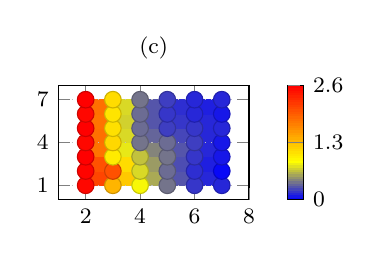
\begin{tikzpicture}
\begin{axis}
[
width=0.33\textwidth,
height=0.25\textwidth,
style={font=\footnotesize},
grid=major,
grid style={dotted},
align=center,
%xlabel={tensor order},
%ylabel={contr. mode (q)},
title={{(c)}}, %  ompfor<qd-slice> ttm<par-loops,seq-blas,$q$-slice>, asymmetric
scaled ticks=false,
zlabel={GFlops},
view={0}{90}, 
ytick={1,4,7,10},
xtick={2,4,6,8},
xmin=1, xmax=8,
ymin=0, ymax=8,
try min ticks=8,
zmin=0, zmax=2600,
point meta min=0, point meta max=2600,
%colormap/jet, 
colormap/hot, 
%colormap/blackwhite,
%colormap={whiteblack}{indices of colormap={\pgfplotscolormaplastindexof{blackwhite},...,0 of blackwhite}},
samples=50,
%colormap access=piecewise const,
colorbar sampled,
colorbar/width=0.2cm,
colorbar style={
point meta min=0, point meta max=2600,
samples=50,
font=\footnotesize,
ytick={0,1300,2600},
yticklabels={0,1.3,2.6},
%title={\scriptsize Gflops},
%ylabel={\scriptsize Gflops},
}
]
%\addplot3[mesh, scatter,samples=50,shader=interp]
%\addplot3[only marks, mesh, scatter,scatter src=z,samples=50,] % z buffer=sort, scatter src=z,
\addplot3[contour filled={number=100},scatter,shader=flat,samples=50]
%\addplot3+[mesh,scatter,shader=flat corner,samples=50, only marks, mark size=2]
coordinates{

(2.000,1.000,2536.639) (2.000,2.000,2549.050) (2.000,3.000,2598.729) (2.000,4.000,2525.744) (2.000,5.000,2590.830) (2.000,6.000,2544.134) (2.000,7.000,2589.762) 

(3.000,1.000,1375.656) (3.000,2.000,2048.636) (3.000,3.000,1013.687) (3.000,4.000,1124.134) (3.000,5.000,1075.977) (3.000,6.000,1052.382) (3.000,7.000,1098.544) 

(4.000,1.000,833.978) (4.000,2.000,732.322) (4.000,3.000,660.833) (4.000,4.000,413.827) (4.000,5.000,368.029) (4.000,6.000,382.244) (4.000,7.000,404.286) 

(5.000,1.000,415.086) (5.000,2.000,368.007) (5.000,3.000,411.465) (5.000,4.000,371.633) (5.000,5.000,212.971) (5.000,6.000,198.100) (5.000,7.000,222.798) 

(6.000,1.000,206.159) (6.000,2.000,156.941) (6.000,3.000,192.783) (6.000,4.000,217.075) (6.000,5.000,186.601) (6.000,6.000,132.454) (6.000,7.000,130.229) 

(7.000,1.000,150.869) (7.000,2.000,27.399) (7.000,3.000,91.695) (7.000,4.000,85.698) (7.000,5.000,132.060) (7.000,6.000,86.740) (7.000,7.000,146.783) 


};
\end{axis}
\end{tikzpicture}

\caption{%
\footnotesize %
Performance maps in double-precision Tflops of the proposed algorithms with varying tensor orders $p$  and contraction modes $q$. 
Tensors are asymmetrically-shaped on the upper plots and symmetrically-shaped on the lower plots.
In (a) and (d) function \tf{<gemm\_batch>} is executed,
in (b) and (e) \tf{<par-loops,seq-gemm>} with tensor slices, %
in (c) and (f) \tf{<par-loops,seq-gemm>} with subtensors.
\label{performance.tlib.contour}
}
\end{figure*}


\begin{figure*}[t]
\centering
%\tikzset{every mark/.append style={scale=1.5}}
\begin{tikzpicture}
\begin{axis}[
height=0.3\textheight,
width=0.49\textwidth,
style={font=\footnotesize},
grid=major,
grid style={dotted},
align=center,
xlabel={Tflops},
ylabel={Cumulative Probability},
ylabel near ticks,
%title={Empirical CDF},
xtick={0,400,800,1200,1600,2000,2400},
xticklabels={0,0.4,0.8,1.2,1.6,2.0,2.4},
ytick={0,0.25,0.5,0.75,1},
yticklabels={0,0.25,0.5,0.75,1},
mark repeat={16},
cycle list name=my exotic tlib case8
]
\addplot%+[line width=1,mark options={scale=2}]
coordinates{(249.878,0.000) (249.878,0.004) (250.498,0.009) (251.198,0.013) (287.282,0.018) (308.210,0.022) (312.900,0.027) (317.790,0.031) (319.745,0.036) (333.535,0.040) (336.000,0.045) (338.491,0.049) (341.216,0.054) (344.786,0.058) (355.143,0.062) (357.986,0.067) (367.907,0.071) (369.580,0.076) (375.479,0.080) (375.729,0.085) (382.059,0.089) (388.669,0.094) (389.946,0.098) (390.969,0.103) (392.443,0.107) (396.968,0.112) (402.255,0.116) (402.307,0.121) (404.538,0.125) (407.716,0.129) (410.815,0.134) (411.312,0.138) (411.358,0.143) (418.596,0.147) (424.356,0.152) (427.055,0.156) (427.234,0.161) (430.656,0.165) (430.884,0.170) (432.740,0.174) (433.748,0.179) (434.447,0.183) (437.092,0.188) (439.283,0.192) (442.064,0.196) (442.284,0.201) (444.761,0.205) (450.271,0.210) (451.374,0.214) (456.669,0.219) (457.774,0.223) (458.702,0.228) (461.089,0.232) (462.931,0.237) (464.799,0.241) (468.844,0.246) (470.529,0.250) (473.086,0.254) (473.916,0.259) (475.694,0.263) (483.246,0.268) (487.229,0.272) (487.714,0.277) (491.142,0.281) (494.656,0.286) (495.606,0.290) (496.699,0.295) (497.201,0.299) (497.747,0.304) (501.887,0.308) (502.643,0.312) (506.654,0.317) (509.707,0.321) (511.859,0.326) (512.660,0.330) (514.424,0.335) (515.081,0.339) (520.970,0.344) (521.336,0.348) (523.241,0.353) (523.382,0.357) (525.138,0.362) (525.357,0.366) (525.433,0.371) (526.644,0.375) (526.940,0.379) (527.210,0.384) (528.215,0.388) (529.222,0.393) (531.310,0.397) (532.989,0.402) (533.334,0.406) (533.663,0.411) (534.694,0.415) (540.081,0.420) (542.065,0.424) (544.215,0.429) (544.947,0.433) (547.123,0.437) (550.597,0.442) (552.140,0.446) (553.837,0.451) (557.286,0.455) (559.484,0.460) (560.642,0.464) (562.740,0.469) (563.396,0.473) (565.032,0.478) (566.862,0.482) (571.435,0.487) (572.451,0.491) (579.442,0.496) (584.946,0.500) (599.990,0.504) (601.535,0.509) (607.596,0.513) (615.585,0.518) (630.732,0.522) (638.927,0.527) (643.727,0.531) (648.221,0.536) (652.873,0.540) (687.371,0.545) (689.520,0.549) (702.614,0.554) (744.308,0.558) (747.150,0.562) (748.599,0.567) (757.094,0.571) (795.624,0.576) (799.079,0.580) (810.978,0.585) (815.722,0.589) (827.278,0.594) (843.004,0.598) (858.076,0.603) (884.822,0.607) (897.720,0.612) (956.927,0.616) (965.241,0.621) (1011.204,0.625) (1046.045,0.629) (1076.318,0.634) (1089.744,0.638) (1197.500,0.643) (1209.389,0.647) (1228.423,0.652) (1242.111,0.656) (1242.587,0.661) (1295.741,0.665) (1308.737,0.670) (1314.667,0.674) (1319.584,0.679) (1324.770,0.683) (1328.634,0.688) (1335.439,0.692) (1335.690,0.696) (1336.527,0.701) (1336.958,0.705) (1337.562,0.710) (1338.761,0.714) (1350.351,0.719) (1366.023,0.723) (1376.231,0.728) (1379.587,0.732) (1414.123,0.737) (1416.843,0.741) (1421.074,0.746) (1424.784,0.750) (1434.474,0.754) (1440.908,0.759) (1447.261,0.763) (1450.436,0.768) (1468.565,0.772) (1470.991,0.777) (1479.798,0.781) (1488.778,0.786) (1499.268,0.790) (1501.348,0.795) (1510.014,0.799) (1513.052,0.804) (1519.239,0.808) (1524.506,0.812) (1529.999,0.817) (1570.936,0.821) (1577.946,0.826) (1585.559,0.830) (1595.181,0.835) (1602.500,0.839) (1619.485,0.844) (1622.265,0.848) (1627.168,0.853) (1630.442,0.857) (1632.244,0.862) (1637.079,0.866) (1642.740,0.871) (1645.993,0.875) (1654.078,0.879) (1663.716,0.884) (1664.997,0.888) (1665.178,0.893) (1670.765,0.897) (1688.335,0.902) (1691.254,0.906) (1718.916,0.911) (1725.607,0.915) (1727.856,0.920) (1731.761,0.924) (1744.728,0.929) (1752.285,0.933) (1756.083,0.938) (1757.644,0.942) (1758.204,0.946) (1768.225,0.951) (1779.870,0.955) (1783.104,0.960) (1788.292,0.964) (1789.250,0.969) (1820.619,0.973) (1839.385,0.978) (1852.487,0.982) (1862.303,0.987) (1863.897,0.991) (1973.525,0.996) (2061.434,1.000) };
%\label{coord_performance_double:5_1}tlib<bgemm,subtensor,all>

\addplot%+[line width=1,mark options={scale=2}]
coordinates{(313.659,0.000) (313.659,0.004) (353.645,0.009) (354.404,0.013) (395.361,0.018) (437.395,0.022) (497.558,0.027) (508.645,0.031) (544.980,0.036) (563.449,0.040) (564.554,0.045) (581.429,0.049) (650.239,0.054) (662.663,0.058) (679.784,0.062) (688.803,0.067) (706.165,0.071) (716.610,0.076) (730.623,0.080) (738.986,0.085) (788.205,0.089) (810.231,0.094) (823.259,0.098) (834.928,0.103) (861.437,0.107) (901.891,0.112) (903.570,0.116) (920.436,0.121) (930.774,0.125) (934.850,0.129) (951.188,0.134) (960.004,0.138) (962.563,0.143) (966.043,0.147) (966.174,0.152) (979.316,0.156) (986.993,0.161) (1009.983,0.165) (1020.452,0.170) (1022.657,0.174) (1028.810,0.179) (1034.272,0.183) (1036.976,0.188) (1050.062,0.192) (1051.796,0.196) (1062.711,0.201) (1067.288,0.205) (1072.511,0.210) (1082.596,0.214) (1088.237,0.219) (1090.330,0.223) (1092.975,0.228) (1102.765,0.232) (1114.497,0.237) (1114.593,0.241) (1122.806,0.246) (1126.217,0.250) (1135.637,0.254) (1137.751,0.259) (1138.835,0.263) (1146.623,0.268) (1147.619,0.272) (1181.353,0.277) (1182.430,0.281) (1184.884,0.286) (1201.905,0.290) (1205.509,0.295) (1207.903,0.299) (1207.903,0.304) (1208.759,0.308) (1215.868,0.312) (1220.133,0.317) (1231.537,0.321) (1238.270,0.326) (1243.584,0.330) (1277.572,0.335) (1283.876,0.339) (1285.151,0.344) (1287.335,0.348) (1298.257,0.353) (1315.811,0.357) (1316.039,0.362) (1366.001,0.366) (1366.897,0.371) (1369.617,0.375) (1376.473,0.379) (1393.366,0.384) (1401.023,0.388) (1422.138,0.393) (1422.885,0.397) (1424.394,0.402) (1424.432,0.406) (1438.882,0.411) (1462.382,0.415) (1463.468,0.420) (1471.482,0.424) (1475.947,0.429) (1480.454,0.433) (1496.047,0.437) (1502.328,0.442) (1503.616,0.446) (1504.874,0.451) (1507.989,0.455) (1516.021,0.460) (1522.187,0.464) (1532.528,0.469) (1539.797,0.473) (1547.642,0.478) (1549.595,0.482) (1557.894,0.487) (1561.675,0.491) (1569.135,0.496) (1569.514,0.500) (1587.092,0.504) (1587.869,0.509) (1591.106,0.513) (1600.096,0.518) (1601.528,0.522) (1605.107,0.527) (1605.151,0.531) (1617.053,0.536) (1620.146,0.540) (1629.690,0.545) (1632.609,0.549) (1632.696,0.554) (1633.275,0.558) (1634.796,0.562) (1637.654,0.567) (1651.681,0.571) (1654.162,0.576) (1665.199,0.580) (1667.639,0.585) (1669.471,0.589) (1674.088,0.594) (1677.796,0.598) (1682.470,0.603) (1682.711,0.607) (1684.516,0.612) (1688.157,0.616) (1691.099,0.621) (1711.546,0.625) (1726.766,0.629) (1760.353,0.634) (1765.300,0.638) (1770.500,0.643) (1783.309,0.647) (1789.882,0.652) (1792.533,0.656) (1795.768,0.661) (1800.116,0.665) (1805.320,0.670) (1807.059,0.674) (1807.821,0.679) (1809.753,0.683) (1810.388,0.688) (1812.495,0.692) (1813.960,0.696) (1814.728,0.701) (1820.099,0.705) (1820.917,0.710) (1824.126,0.714) (1825.413,0.719) (1825.684,0.723) (1825.721,0.728) (1827.673,0.732) (1827.970,0.737) (1828.344,0.741) (1836.431,0.746) (1837.992,0.750) (1839.444,0.754) (1839.503,0.759) (1841.563,0.763) (1845.372,0.768) (1845.998,0.772) (1846.046,0.777) (1849.786,0.781) (1850.187,0.786) (1851.203,0.790) (1851.540,0.795) (1852.859,0.799) (1856.015,0.804) (1856.955,0.808) (1857.069,0.812) (1859.505,0.817) (1860.936,0.821) (1861.310,0.826) (1864.998,0.830) (1866.287,0.835) (1868.883,0.839) (1870.073,0.844) (1870.293,0.848) (1872.809,0.853) (1873.115,0.857) (1875.101,0.862) (1875.432,0.866) (1875.581,0.871) (1877.757,0.875) (1877.982,0.879) (1878.414,0.884) (1879.894,0.888) (1880.045,0.893) (1880.450,0.897) (1881.113,0.902) (1881.393,0.906) (1884.000,0.911) (1887.361,0.915) (1889.667,0.920) (1890.892,0.924) (1891.194,0.929) (1892.197,0.933) (1894.496,0.938) (1902.227,0.942) (1915.959,0.946) (1919.571,0.951) (1921.120,0.955) (1931.400,0.960) (1946.799,0.964) (1956.869,0.969) (1962.895,0.973) (1977.326,0.978) (1996.608,0.982) (2018.941,0.987) (2037.235,0.991) (2040.283,0.996) (2074.004,1.000) };
%\label{coord_performance_double:4_1} tlib<tgemm,slice>

\addplot%+[line width=1,mark options={scale=2}]
coordinates{(276.757,0.000) (276.757,0.004) (289.438,0.009) (309.721,0.013) (319.255,0.018) (322.873,0.022) (328.252,0.027) (332.907,0.031) (335.093,0.036) (441.542,0.040) (453.160,0.045) (478.586,0.049) (541.129,0.054) (541.356,0.058) (542.749,0.062) (543.755,0.067) (545.199,0.071) (545.531,0.076) (568.284,0.080) (573.530,0.085) (587.488,0.089) (588.102,0.094) (589.450,0.098) (592.653,0.103) (604.239,0.107) (610.157,0.112) (611.767,0.116) (616.528,0.121) (617.075,0.125) (618.978,0.129) (663.603,0.134) (707.018,0.138) (885.419,0.143) (961.050,0.147) (972.266,0.152) (989.129,0.156) (1002.446,0.161) (1008.069,0.165) (1008.831,0.170) (1010.252,0.174) (1011.281,0.179) (1014.055,0.183) (1019.924,0.188) (1022.241,0.192) (1026.660,0.196) (1027.502,0.201) (1028.538,0.205) (1029.795,0.210) (1031.782,0.214) (1036.111,0.219) (1043.064,0.223) (1044.256,0.228) (1044.905,0.232) (1052.021,0.237) (1056.395,0.241) (1063.336,0.246) (1080.738,0.250) (1091.013,0.254) (1095.898,0.259) (1101.527,0.263) (1102.111,0.268) (1135.046,0.272) (1142.434,0.277) (1186.388,0.281) (1229.219,0.286) (1248.102,0.290) (1293.153,0.295) (1297.057,0.299) (1308.856,0.304) (1310.097,0.308) (1354.309,0.312) (1367.741,0.317) (1376.234,0.321) (1381.238,0.326) (1383.584,0.330) (1419.043,0.335) (1420.828,0.339) (1420.940,0.344) (1450.631,0.348) (1488.938,0.353) (1489.646,0.357) (1497.275,0.362) (1500.888,0.366) (1503.266,0.371) (1506.950,0.375) (1523.595,0.379) (1528.489,0.384) (1529.138,0.388) (1534.708,0.393) (1542.806,0.397) (1554.439,0.402) (1554.581,0.406) (1557.493,0.411) (1564.443,0.415) (1572.957,0.420) (1573.367,0.424) (1574.950,0.429) (1577.375,0.433) (1578.258,0.437) (1596.822,0.442) (1599.083,0.446) (1601.277,0.451) (1601.533,0.455) (1619.975,0.460) (1620.606,0.464) (1620.747,0.469) (1622.735,0.473) (1624.541,0.478) (1628.113,0.482) (1633.361,0.487) (1633.918,0.491) (1634.861,0.496) (1637.680,0.500) (1638.334,0.504) (1640.251,0.509) (1640.785,0.513) (1642.334,0.518) (1643.994,0.522) (1645.910,0.527) (1648.521,0.531) (1652.740,0.536) (1656.668,0.540) (1658.249,0.545) (1660.699,0.549) (1661.492,0.554) (1662.537,0.558) (1665.239,0.562) (1673.752,0.567) (1676.364,0.571) (1678.376,0.576) (1679.220,0.580) (1679.956,0.585) (1687.436,0.589) (1691.829,0.594) (1693.634,0.598) (1695.376,0.603) (1695.775,0.607) (1698.767,0.612) (1701.879,0.616) (1707.420,0.621) (1709.013,0.625) (1710.273,0.629) (1714.385,0.634) (1716.980,0.638) (1718.576,0.643) (1718.983,0.647) (1719.823,0.652) (1722.670,0.656) (1725.168,0.661) (1725.471,0.665) (1731.858,0.670) (1735.377,0.674) (1735.895,0.679) (1742.512,0.683) (1748.047,0.688) (1748.660,0.692) (1750.481,0.696) (1751.993,0.701) (1758.709,0.705) (1761.181,0.710) (1762.953,0.714) (1766.562,0.719) (1767.541,0.723) (1768.620,0.728) (1770.963,0.732) (1772.173,0.737) (1775.667,0.741) (1783.859,0.746) (1794.472,0.750) (1795.810,0.754) (1798.827,0.759) (1799.282,0.763) (1831.730,0.768) (1837.013,0.772) (1837.374,0.777) (1842.893,0.781) (1855.814,0.786) (1857.034,0.790) (1863.211,0.795) (1866.512,0.799) (1874.637,0.804) (1879.106,0.808) (1879.949,0.812) (1893.562,0.817) (1918.258,0.821) (1921.485,0.826) (1925.062,0.830) (1927.188,0.835) (1929.594,0.839) (1932.643,0.844) (1941.205,0.848) (1947.687,0.853) (1950.634,0.857) (1952.378,0.862) (1955.973,0.866) (1962.611,0.871) (1963.898,0.875) (1975.705,0.879) (1977.796,0.884) (1985.281,0.888) (1985.764,0.893) (1991.141,0.897) (2004.006,0.902) (2015.463,0.906) (2020.675,0.911) (2021.342,0.915) (2037.183,0.920) (2042.126,0.924) (2043.565,0.929) (2052.795,0.933) (2061.290,0.938) (2085.577,0.942) (2091.541,0.946) (2107.633,0.951) (2122.542,0.955) (2129.293,0.960) (2144.986,0.964) (2146.823,0.969) (2149.982,0.973) (2173.440,0.978) (2178.995,0.982) (2182.289,0.987) (2214.990,0.991) (2220.201,0.996) (2224.984,1.000) };
%\label{coord_performance_double:1_1}tlib<ompfor,slice,all>


\addplot%+[line width=1,mark options={scale=2}]
coordinates{(371.830,0.000) (371.830,0.004) (389.393,0.009) (438.032,0.013) (495.113,0.018) (541.464,0.022) (554.114,0.027) (571.666,0.031) (726.325,0.036) (758.146,0.040) (856.111,0.045) (856.916,0.049) (876.422,0.054) (878.126,0.058) (886.409,0.062) (911.886,0.067) (915.260,0.071) (946.712,0.076) (957.481,0.080) (986.357,0.085) (989.711,0.089) (990.142,0.094) (1011.101,0.098) (1018.471,0.103) (1021.812,0.107) (1025.632,0.112) (1074.521,0.116) (1089.495,0.121) (1102.427,0.125) (1124.158,0.129) (1126.558,0.134) (1136.932,0.138) (1141.223,0.143) (1144.221,0.147) (1145.378,0.152) (1155.193,0.156) (1155.766,0.161) (1161.337,0.165) (1165.452,0.170) (1171.885,0.174) (1210.222,0.179) (1225.256,0.183) (1232.484,0.188) (1258.931,0.192) (1262.358,0.196) (1284.512,0.201) (1312.955,0.205) (1322.956,0.210) (1324.739,0.214) (1336.964,0.219) (1343.700,0.223) (1345.076,0.228) (1350.681,0.232) (1353.054,0.237) (1356.408,0.241) (1360.679,0.246) (1363.866,0.250) (1369.790,0.254) (1387.001,0.259) (1398.949,0.263) (1399.346,0.268) (1410.702,0.272) (1416.124,0.277) (1419.661,0.281) (1422.766,0.286) (1423.876,0.290) (1431.656,0.295) (1434.486,0.299) (1436.657,0.304) (1443.949,0.308) (1447.560,0.312) (1451.425,0.317) (1451.449,0.321) (1455.698,0.326) (1476.320,0.330) (1484.316,0.335) (1486.764,0.339) (1491.693,0.344) (1498.989,0.348) (1513.885,0.353) (1515.937,0.357) (1527.310,0.362) (1527.955,0.366) (1537.175,0.371) (1537.420,0.375) (1550.070,0.379) (1571.097,0.384) (1578.270,0.388) (1581.378,0.393) (1581.385,0.397) (1582.667,0.402) (1590.563,0.406) (1597.607,0.411) (1599.349,0.415) (1619.749,0.420) (1622.248,0.424) (1622.350,0.429) (1622.717,0.433) (1629.413,0.437) (1647.445,0.442) (1648.940,0.446) (1654.452,0.451) (1660.166,0.455) (1660.891,0.460) (1664.070,0.464) (1665.360,0.469) (1678.021,0.473) (1678.326,0.478) (1679.870,0.482) (1680.546,0.487) (1683.200,0.491) (1691.316,0.496) (1699.737,0.500) (1699.951,0.504) (1701.525,0.509) (1706.578,0.513) (1706.925,0.518) (1707.133,0.522) (1710.737,0.527) (1713.593,0.531) (1725.529,0.536) (1741.188,0.540) (1746.114,0.545) (1755.454,0.549) (1760.797,0.554) (1771.081,0.558) (1776.264,0.562) (1776.406,0.567) (1787.293,0.571) (1788.168,0.576) (1789.482,0.580) (1792.099,0.585) (1798.005,0.589) (1800.322,0.594) (1801.849,0.598) (1807.746,0.603) (1808.961,0.607) (1809.533,0.612) (1818.377,0.616) (1821.344,0.621) (1825.493,0.625) (1830.431,0.629) (1830.449,0.634) (1831.024,0.638) (1844.509,0.643) (1844.705,0.647) (1848.600,0.652) (1869.812,0.656) (1871.770,0.661) (1873.026,0.665) (1873.302,0.670) (1875.887,0.674) (1875.980,0.679) (1876.313,0.683) (1877.565,0.688) (1879.735,0.692) (1880.428,0.696) (1884.544,0.701) (1887.179,0.705) (1887.989,0.710) (1890.330,0.714) (1893.422,0.719) (1894.675,0.723) (1894.987,0.728) (1897.598,0.732) (1898.233,0.737) (1901.227,0.741) (1904.073,0.746) (1904.786,0.750) (1906.302,0.754) (1907.476,0.759) (1907.926,0.763) (1908.127,0.768) (1908.619,0.772) (1915.191,0.777) (1924.349,0.781) (1925.867,0.786) (1931.020,0.790) (1931.121,0.795) (1933.098,0.799) (1933.605,0.804) (1934.785,0.808) (1936.904,0.812) (1937.146,0.817) (1937.263,0.821) (1939.428,0.826) (1943.576,0.830) (1948.572,0.835) (1949.583,0.839) (1950.797,0.844) (1953.635,0.848) (1956.826,0.853) (1957.158,0.857) (1957.439,0.862) (1958.407,0.866) (1959.901,0.871) (1962.339,0.875) (1964.007,0.879) (1965.495,0.884) (1968.832,0.888) (1969.274,0.893) (1970.258,0.897) (1970.264,0.902) (1970.386,0.906) (1973.368,0.911) (1974.246,0.915) (1974.543,0.920) (1975.168,0.924) (1975.297,0.929) (1975.833,0.933) (1977.011,0.938) (1980.963,0.942) (1985.398,0.946) (1988.229,0.951) (1993.241,0.955) (1996.726,0.960) (1997.228,0.964) (1997.616,0.969) (2001.286,0.973) (2002.667,0.978) (2002.754,0.982) (2008.661,0.987) (2018.425,0.991) (2032.035,0.996) (2057.768,1.000) };
%\label{coord_performance_double:3_1}tlib<tgemm,subtensor>\\



\addplot%+[line width=1,mark options={scale=2}]
coordinates{(119.981,0.000) (119.981,0.004) (186.838,0.009) (187.551,0.013) (187.833,0.018) (230.722,0.022) (235.685,0.027) (236.533,0.031) (244.309,0.036) (252.881,0.040) (253.937,0.045) (255.615,0.049) (257.832,0.054) (270.106,0.058) (270.177,0.062) (271.350,0.067) (271.678,0.071) (275.559,0.076) (276.291,0.080) (276.987,0.085) (281.873,0.089) (281.876,0.094) (281.963,0.098) (285.445,0.103) (286.075,0.107) (286.241,0.112) (288.097,0.116) (288.184,0.121) (288.894,0.125) (290.020,0.129) (290.104,0.134) (291.685,0.138) (293.698,0.143) (294.302,0.147) (297.020,0.152) (298.110,0.156) (300.594,0.161) (303.274,0.165) (303.960,0.170) (304.154,0.174) (304.911,0.179) (305.212,0.183) (309.709,0.188) (311.565,0.192) (313.122,0.196) (313.867,0.201) (319.339,0.205) (321.016,0.210) (326.052,0.214) (329.252,0.219) (329.405,0.223) (329.489,0.228) (332.219,0.232) (333.671,0.237) (333.800,0.241) (335.097,0.246) (336.290,0.250) (336.602,0.254) (336.848,0.259) (338.218,0.263) (362.225,0.268) (400.952,0.272) (429.876,0.277) (445.194,0.281) (455.019,0.286) (459.722,0.290) (474.332,0.295) (478.138,0.299) (479.034,0.304) (485.410,0.308) (493.309,0.312) (495.664,0.317) (496.364,0.321) (501.438,0.326) (502.520,0.330) (508.201,0.335) (515.049,0.339) (521.258,0.344) (523.245,0.348) (526.439,0.353) (528.190,0.357) (534.540,0.362) (534.671,0.366) (542.293,0.371) (542.633,0.375) (543.791,0.379) (549.061,0.384) (549.843,0.388) (555.523,0.393) (557.931,0.397) (568.232,0.402) (571.507,0.406) (575.243,0.411) (575.402,0.415) (575.768,0.420) (580.075,0.424) (582.920,0.429) (586.888,0.433) (589.295,0.437) (592.176,0.442) (604.753,0.446) (609.549,0.451) (609.718,0.455) (614.474,0.460) (615.169,0.464) (617.486,0.469) (618.456,0.473) (624.183,0.478) (625.588,0.482) (626.071,0.487) (631.932,0.491) (705.528,0.496) (721.243,0.500) (758.010,0.504) (778.297,0.509) (806.393,0.513) (829.517,0.518) (836.843,0.522) (855.814,0.527) (861.502,0.531) (866.653,0.536) (894.699,0.540) (897.945,0.545) (903.416,0.549) (903.765,0.554) (910.164,0.558) (911.603,0.562) (931.862,0.567) (961.965,0.571) (972.951,0.576) (985.427,0.580) (1004.418,0.585) (1007.466,0.589) (1007.833,0.594) (1013.539,0.598) (1015.220,0.603) (1024.560,0.607) (1024.791,0.612) (1027.009,0.616) (1028.622,0.621) (1030.777,0.625) (1031.005,0.629) (1033.449,0.634) (1034.617,0.638) (1035.387,0.643) (1038.228,0.647) (1043.742,0.652) (1064.420,0.656) (1064.988,0.661) (1084.427,0.665) (1088.369,0.670) (1101.473,0.674) (1103.975,0.679) (1124.782,0.683) (1153.483,0.688) (1223.548,0.692) (1306.473,0.696) (1344.402,0.701) (1346.315,0.705) (1347.000,0.710) (1354.645,0.714) (1362.804,0.719) (1373.310,0.723) (1393.407,0.728) (1416.909,0.732) (1432.303,0.737) (1447.026,0.741) (1449.835,0.746) (1458.553,0.750) (1460.886,0.754) (1487.709,0.759) (1505.467,0.763) (1536.144,0.768) (1543.753,0.772) (1546.866,0.777) (1551.101,0.781) (1555.375,0.786) (1557.869,0.790) (1558.782,0.795) (1560.847,0.799) (1585.537,0.804) (1591.449,0.808) (1602.854,0.812) (1604.271,0.817) (1607.143,0.821) (1617.606,0.826) (1617.935,0.830) (1622.699,0.835) (1625.013,0.839) (1642.201,0.844) (1643.039,0.848) (1658.849,0.853) (1685.502,0.857) (1692.709,0.862) (1701.473,0.866) (1713.601,0.871) (1715.570,0.875) (1719.084,0.879) (1719.818,0.884) (1720.810,0.888) (1733.561,0.893) (1743.486,0.897) (1749.358,0.902) (1750.911,0.906) (1754.582,0.911) (1767.663,0.915) (1796.456,0.920) (1801.299,0.924) (1880.126,0.929) (1888.357,0.933) (1907.355,0.938) (1944.024,0.942) (1981.750,0.946) (1984.979,0.951) (1987.458,0.955) (1989.743,0.960) (2039.365,0.964) (2089.299,0.969) (2119.371,0.973) (2132.838,0.978) (2133.321,0.982) (2183.575,0.987) (2216.024,0.991) (2234.394,0.996) (2236.967,1.000) };
%\label{coord_performance_double:2_1}tlib<ompfor,subtensor,all>



\end{axis}
\end{tikzpicture}
\hfill
\begin{tikzpicture}
\begin{axis}[
height=0.3\textheight,
width=0.49\textwidth,
style={font=\footnotesize},
grid=major,
grid style={dotted},
align=center,
xlabel={Tflops},
ylabel={Cumulative Probability},
ylabel near ticks,
ytick={0,0.25,0.5,0.75,1},
yticklabels={0,0.25,0.5,0.75,1},
title={},
xtick={0,200,400,600,800,1000},
xticklabels={0,0.2,0.4,0.6,0.8,1},
mark repeat={4},
cycle list name=my exotic tlib case8
]

\addplot
coordinates{(14.818,0.000) (14.818,0.011) (19.140,0.022) (24.958,0.033) (25.392,0.044) (30.008,0.056) (35.416,0.067) (38.901,0.078) (51.622,0.089) (58.276,0.100) (63.435,0.111) (66.233,0.122) (70.884,0.133) (73.671,0.144) (78.935,0.156) (81.951,0.167) (82.141,0.178) (87.214,0.189) (90.980,0.200) (94.040,0.211) (94.208,0.222) (94.947,0.233) (95.250,0.244) (97.652,0.256) (101.138,0.267) (101.566,0.278) (104.614,0.289) (105.150,0.300) (107.716,0.311) (107.804,0.322) (110.412,0.333) (110.489,0.344) (112.046,0.356) (116.361,0.367) (117.149,0.378) (120.622,0.389) (124.229,0.400) (126.456,0.411) (128.850,0.422) (130.301,0.433) (134.515,0.444) (141.163,0.456) (144.718,0.467) (147.126,0.478) (151.629,0.489) (153.604,0.500) (156.699,0.511) (157.858,0.522) (160.142,0.533) (170.440,0.544) (174.354,0.556) (182.941,0.567) (183.971,0.578) (186.642,0.589) (194.103,0.600) (195.452,0.611) (197.366,0.622) (198.047,0.633) (215.920,0.644) (222.558,0.656) (223.415,0.667) (231.493,0.678) (235.199,0.689) (235.771,0.700) (240.725,0.711) (251.213,0.722) (278.183,0.733) (290.902,0.744) (291.032,0.756) (300.677,0.767) (311.011,0.778) (327.432,0.789) (330.011,0.800) (336.634,0.811) (356.805,0.822) (364.975,0.833) (394.036,0.844) (406.761,0.856) (429.050,0.867) (433.063,0.878) (435.655,0.889) (451.363,0.900) (506.258,0.911) (557.079,0.922) (574.476,0.933) (598.644,0.944) (640.269,0.956) (673.482,0.967) (692.468,0.978) (866.633,0.989) (900.345,1.000) };
\label{coord:gemm_batch} % tlib<bgemm,subtensor,all>

\addplot
coordinates{(3.514,0.000) (3.514,0.011) (3.956,0.022) (4.026,0.033) (4.217,0.044) (4.302,0.056) (5.014,0.067) (5.759,0.078) (5.763,0.089) (6.020,0.100) (6.543,0.111) (6.731,0.122) (7.709,0.133) (7.952,0.144) (8.050,0.156) (8.444,0.167) (9.312,0.178) (9.495,0.189) (9.849,0.200) (10.329,0.211) (10.358,0.222) (11.423,0.233) (11.883,0.244) (11.943,0.256) (13.404,0.267) (14.361,0.278) (14.764,0.289) (15.016,0.300) (15.071,0.311) (15.169,0.322) (15.893,0.333) (16.403,0.344) (16.701,0.356) (16.780,0.367) (17.144,0.378) (17.224,0.389) (17.239,0.400) (17.540,0.411) (17.814,0.422) (17.890,0.433) (18.912,0.444) (19.348,0.456) (20.546,0.467) (21.039,0.478) (23.875,0.489) (26.289,0.500) (26.926,0.511) (27.516,0.522) (27.889,0.533) (28.234,0.544) (29.405,0.556) (29.419,0.567) (29.761,0.578) (31.392,0.589) (31.810,0.600) (32.159,0.611) (32.169,0.622) (32.388,0.633) (33.286,0.644) (33.485,0.656) (33.496,0.667) (33.537,0.678) (34.487,0.689) (34.736,0.700) (35.070,0.711) (35.539,0.722) (35.855,0.733) (35.895,0.744) (36.008,0.756) (36.202,0.767) (36.537,0.778) (37.063,0.789) (38.165,0.800) (38.294,0.811) (38.829,0.822) (42.533,0.833) (42.669,0.844) (42.700,0.856) (44.461,0.867) (48.007,0.878) (55.190,0.889) (58.417,0.900) (65.084,0.911) (89.844,0.922) (96.283,0.933) (115.682,0.944) (148.213,0.956) (173.663,0.967) (211.622,0.978) (269.857,0.989) (274.254,1.000) };
\label{coord:seq_loops_par_gemm_slice} %tlib<tgemm,slice>

\addplot
coordinates{(7.389,0.000) (7.389,0.011) (7.712,0.022) (8.807,0.033) (9.117,0.044) (10.708,0.056) (10.822,0.067) (12.116,0.078) (12.576,0.089) (14.483,0.100) (14.925,0.111) (16.809,0.122) (17.316,0.133) (18.888,0.144) (19.629,0.156) (21.799,0.167) (22.502,0.178) (22.782,0.189) (26.323,0.200) (27.705,0.211) (27.713,0.222) (31.204,0.233) (34.932,0.244) (35.675,0.256) (35.891,0.267) (39.050,0.278) (43.477,0.289) (44.145,0.300) (44.446,0.311) (46.536,0.322) (51.986,0.333) (52.474,0.344) (53.209,0.356) (53.989,0.367) (55.059,0.378) (55.257,0.389) (58.433,0.400) (59.480,0.411) (61.548,0.422) (62.750,0.433) (77.043,0.444) (83.618,0.456) (87.516,0.467) (95.385,0.478) (101.893,0.489) (107.480,0.500) (107.506,0.511) (115.606,0.522) (118.594,0.533) (127.594,0.544) (134.359,0.556) (150.598,0.567) (152.097,0.578) (156.023,0.589) (158.439,0.600) (166.760,0.611) (176.759,0.622) (186.894,0.633) (189.870,0.644) (190.564,0.656) (194.193,0.667) (200.396,0.678) (212.421,0.689) (232.464,0.700) (236.494,0.711) (256.710,0.722) (260.391,0.733) (262.521,0.744) (279.138,0.756) (285.259,0.767) (288.847,0.778) (317.975,0.789) (321.800,0.800) (328.962,0.811) (344.494,0.822) (370.351,0.833) (371.879,0.844) (386.761,0.856) (394.042,0.867) (425.909,0.878) (443.885,0.889) (476.238,0.900) (507.294,0.911) (547.875,0.922) (603.911,0.933) (647.681,0.944) (717.045,0.956) (774.667,0.967) (864.930,0.978) (940.723,0.989) (959.956,1.000) };
\label{coord:par_loops_seq_gemm_slice} %tlib<ompfor,slice,all>


\addplot
coordinates{(5.449,0.000) (5.449,0.011) (6.383,0.022) (6.647,0.033) (8.083,0.044) (9.791,0.056) (11.330,0.067) (11.396,0.078) (11.439,0.089) (11.993,0.100) (12.403,0.111) (13.424,0.122) (13.877,0.133) (15.121,0.144) (15.279,0.156) (15.576,0.167) (16.084,0.178) (16.104,0.189) (16.837,0.200) (16.954,0.211) (17.616,0.222) (17.642,0.233) (17.796,0.244) (17.934,0.256) (18.891,0.267) (18.967,0.278) (19.233,0.289) (19.637,0.300) (20.598,0.311) (21.464,0.322) (21.964,0.333) (23.161,0.344) (23.337,0.356) (23.915,0.367) (24.071,0.378) (27.336,0.389) (27.612,0.400) (27.713,0.411) (29.546,0.422) (31.952,0.433) (33.060,0.444) (33.364,0.456) (33.668,0.467) (35.026,0.478) (35.970,0.489) (38.100,0.500) (39.490,0.511) (42.313,0.522) (42.527,0.533) (42.728,0.544) (42.769,0.556) (46.652,0.567) (48.005,0.578) (50.770,0.589) (52.371,0.600) (52.426,0.611) (53.153,0.622) (57.197,0.633) (58.354,0.644) (59.655,0.656) (62.440,0.667) (66.563,0.678) (78.965,0.689) (79.329,0.700) (79.409,0.711) (82.203,0.722) (84.166,0.733) (85.966,0.744) (86.600,0.756) (88.912,0.767) (91.147,0.778) (95.004,0.789) (104.868,0.800) (110.656,0.811) (129.814,0.822) (133.072,0.833) (148.047,0.844) (155.186,0.856) (165.127,0.867) (174.193,0.878) (175.350,0.889) (192.467,0.900) (204.272,0.911) (213.832,0.922) (234.397,0.933) (234.582,0.944) (236.908,0.956) (241.535,0.967) (243.965,0.978) (271.690,0.989) (317.589,1.000) };
\label{coord:seq_loops_par_gemm_subtensor} %tlib<tgemm,subtensor>

\addplot
coordinates{(7.414,0.000) (7.414,0.011) (8.720,0.022) (10.657,0.033) (14.445,0.044) (18.865,0.056) (24.158,0.067) (28.146,0.078) (30.684,0.089) (38.939,0.100) (44.470,0.111) (46.850,0.122) (54.582,0.133) (55.681,0.144) (55.693,0.156) (77.088,0.167) (85.320,0.178) (86.573,0.189) (87.516,0.200) (91.660,0.211) (94.978,0.222) (95.683,0.233) (96.983,0.244) (100.328,0.256) (102.221,0.267) (108.210,0.278) (110.342,0.289) (112.143,0.300) (113.348,0.311) (114.980,0.322) (115.840,0.333) (118.713,0.344) (119.625,0.356) (128.386,0.367) (128.526,0.378) (129.480,0.389) (130.513,0.400) (133.604,0.411) (135.582,0.422) (139.840,0.433) (145.563,0.444) (146.885,0.456) (149.455,0.467) (156.244,0.478) (169.008,0.489) (169.040,0.500) (171.874,0.511) (174.269,0.522) (184.481,0.533) (184.519,0.544) (185.551,0.556) (203.706,0.567) (209.585,0.578) (210.930,0.589) (212.508,0.600) (224.066,0.611) (230.996,0.622) (234.972,0.633) (236.839,0.644) (249.532,0.656) (257.927,0.667) (259.387,0.678) (262.559,0.689) (275.610,0.700) (286.144,0.711) (289.957,0.722) (295.668,0.733) (302.406,0.744) (317.627,0.756) (341.280,0.767) (343.272,0.778) (372.071,0.789) (383.914,0.800) (394.994,0.811) (418.146,0.822) (427.883,0.833) (441.195,0.844) (452.695,0.856) (458.648,0.867) (479.232,0.878) (501.651,0.889) (514.603,0.900) (539.044,0.911) (555.552,0.922) (604.949,0.933) (654.801,0.944) (718.280,0.956) (789.951,0.967) (868.589,0.978) (931.979,0.989) (952.191,1.000) };
\label{coord:par_loops_seq_gemm_subtensor} %tlib<ompfor,subtensor,all>


\end{axis}
\end{tikzpicture} % boxplot
\caption{ %
\footnotesize%
Cumulative performance distributions of the proposed algorithms for the eighth case.
Each distribution line belongs to one algorithm:
\tf{<gemm\_batch>} \ref{coord:gemm_batch} , %
\tf{<seq-loops,par-gemm>} (\ref{coord:seq_loops_par_gemm_slice}) and
\tf{<par-loops,seq-gemm>} (\ref{coord:par_loops_seq_gemm_slice}) using tensor slices,
\tf{<seq-loops,par-gemm>} (\ref{coord:seq_loops_par_gemm_subtensor}) and
\tf{<par-loops,seq-gemm>} (\ref{coord:par_loops_seq_gemm_subtensor}) using subtensors.
Tensors are asymmetrically (left plot) and symmetrically shaped (right plot).
}
\label{fig:performance.tlib.case8}
\end{figure*}


\begin{figure*}[t]
\begin{tikzpicture}
\begin{axis}[
boxplot/draw direction=y,
width=0.5\textwidth,
height=0.3\textheight,
style={font=\footnotesize},
grid=major,
grid style={dotted},
align=center,
xlabel={$k$-order layout},
ylabel={TFlops},
ylabel near ticks,
%title={Performance (Tflops/s)},
xtick={1,2,3,4,5,6,7},
xticklabels={1,2,3,4,5,6,7},
ymin=0,
ymax=200,
ytick={0,100,200},
yticklabels={0,0.1,0.2},
cycle list={{black}},
boxplot/variable width,
boxplot/box extend=0.5,
boxplot/every box/.style={fill=black,thick},
boxplot/every median/.style={draw=white,thin},
]
\addplot+[boxplot prepared={lower whisker = 12.953287, lower quartile = 60.316441, median = 75.006325, upper quartile = 89.433827, upper whisker = 117.121454} ] coordinates{};
\addplot+[boxplot prepared={lower whisker = 12.640045, lower quartile = 48.857803, median = 71.928801, upper quartile = 83.642690, upper whisker = 129.266128} ] coordinates{};
\addplot+[boxplot prepared={lower whisker = 11.285366, lower quartile = 38.052710, median = 47.911392, upper quartile = 58.133262, upper whisker = 82.945640} ] coordinates{};
\addplot+[boxplot prepared={lower whisker = 15.226172, lower quartile = 57.231846, median = 80.633181, upper quartile = 93.816564, upper whisker = 183.850079} ] coordinates{};
\addplot+[boxplot prepared={lower whisker = 14.986315, lower quartile = 49.549662, median = 65.947492, upper quartile = 82.637276, upper whisker = 134.213232} ] coordinates{};
\addplot+[boxplot prepared={lower whisker = 10.126218, lower quartile = 48.886168, median = 65.468008, upper quartile = 78.704242, upper whisker = 142.986427} ] coordinates{};
\addplot+[boxplot prepared={lower whisker = 9.920391, lower quartile = 46.556304, median = 53.812431, upper quartile = 67.449759, upper whisker = 97.531103} ] coordinates{};
\end{axis}
\end{tikzpicture}
\hfill
\begin{tikzpicture}
\begin{axis}[
boxplot/draw direction=y,
width=0.5\textwidth,
height=0.3\textheight,
style={font=\footnotesize},
grid=major,
grid style={dotted},
align=center,
xlabel={$k$-order layout},
%xlabel={Function},
ylabel={TFlops},
ylabel near ticks,
%title={Performance (Tflops/s)},
xtick={1,2,3,4,5,6,7},
xticklabels={1,2,3,4,5,6,7},
ymin=0,
ymax=200,
ytick={0,100,200},
yticklabels={0,0.1,0.2},
cycle list={{black}},
boxplot/variable width,
boxplot/box extend=0.5,
boxplot/every box/.style={fill=black,thick},
boxplot/every median/.style={draw=white,thin},
]
\addplot+[boxplot prepared={lower whisker = 9.972735, lower quartile = 50.927006, median = 64.426586, upper quartile = 79.210059, upper whisker = 102.890428} ] coordinates{};
\addplot+[boxplot prepared={lower whisker = 9.924992, lower quartile = 53.823097, median = 66.585367, upper quartile = 76.424392, upper whisker = 126.976560} ] coordinates{};
\addplot+[boxplot prepared={lower whisker = 9.870402, lower quartile = 40.752707, median = 53.587394, upper quartile = 66.305725, upper whisker = 101.453234} ] coordinates{};
\addplot+[boxplot prepared={lower whisker = 14.708473, lower quartile = 68.924818, median = 80.163598, upper quartile = 97.636473, upper whisker = 172.275314} ] coordinates{};
\addplot+[boxplot prepared={lower whisker = 13.901132, lower quartile = 56.095772, median = 71.850410, upper quartile = 87.921333, upper whisker = 133.760673} ] coordinates{};
\addplot+[boxplot prepared={lower whisker = 9.637782, lower quartile = 64.849736, median = 77.669292, upper quartile = 95.936764, upper whisker = 142.318829} ] coordinates{};
\addplot+[boxplot prepared={lower whisker = 8.748652, lower quartile = 51.209701, median = 67.054182, upper quartile = 87.504879, upper whisker = 115.340741} ] coordinates{};
\end{axis}
\end{tikzpicture}
\begin{comment}
\begin{tikzpicture}
\begin{axis}[
boxplot/draw direction=y,
width=0.37\textwidth,
height=0.3\textheight,
style={font=\footnotesize},
grid=major,
grid style={dotted},
align=center,
xlabel={$k$-order layout},
%xlabel={Function},
%ylabel={Gflops},
%ylabel near ticks,
%title={},
xtick={1,2,3,4,5,6,7},
xticklabels={1,2,3,4,5,6,7},
ymin=0,
ymax=200,
ytick={0,100,200},
yticklabels={0,0.1,0.2},
cycle list={{black}},
boxplot/variable width,
boxplot/box extend=0.5,
boxplot/every box/.style={fill=black,thick},
boxplot/every median/.style={draw=white,thin},
]
\addplot+[boxplot prepared={lower whisker = 7.132722, lower quartile = 11.482166, median = 22.426546, upper quartile = 34.658759, upper whisker = 102.949746} ] coordinates{};
\addplot+[boxplot prepared={lower whisker = 6.479361, lower quartile = 14.151379, median = 27.103188, upper quartile = 40.479719, upper whisker = 97.896991} ] coordinates{};
\addplot+[boxplot prepared={lower whisker = 6.588109, lower quartile = 14.269192, median = 27.672456, upper quartile = 47.110864, upper whisker = 76.267702} ] coordinates{};
\addplot+[boxplot prepared={lower whisker = 10.384620, lower quartile = 19.559000, median = 36.409643, upper quartile = 56.801437, upper whisker = 115.192574} ] coordinates{};
\addplot+[boxplot prepared={lower whisker = 9.428007, lower quartile = 18.814353, median = 35.234564, upper quartile = 50.282299, upper whisker = 93.764754} ] coordinates{};
\addplot+[boxplot prepared={lower whisker = 8.495888, lower quartile = 18.190874, median = 34.228483, upper quartile = 68.448730, upper whisker = 110.241613} ] coordinates{};
\addplot+[boxplot prepared={lower whisker = 7.307545, lower quartile = 16.797509, median = 31.145092, upper quartile = 47.293157, upper whisker = 95.475018} ] coordinates{};
\end{axis}
\end{tikzpicture}
\end{comment}
\caption{ %
\footnotesize%
Box plots visualizing performance statics in double-precision Tflops of \tf{<gemm\_batch>} (left) and \tf{<par-loops,seq-gemm>} with subtensors (right).
Box plot number $k$ denotes the $k$-order tensor layout of symmetrically shaped tensors with order $7$.
% where the $1$-order and $7$-order layouts are the first- and last-order storage formats, respectively.
}
\label{fig:performance.tlib.format}
\end{figure*}

\begin{figure*}[t]
\centering
\tikzset{every mark/.append style={scale=1.5}}
\begin{tikzpicture}
\begin{axis}[
height=0.3\textheight,
width=0.5\textwidth,
style={font=\footnotesize},
grid=major,
grid style={dotted},
align=center,
xlabel={Tflops/s},
ylabel={Cumulative Probability},
ylabel near ticks,
%title={Empirical CDF},
xtick={0,200,400,600,800,1000,1200},
xticklabels={0,0.2,0.4,0.6,0.8,1.0,1.2},
ytick={0,0.25,0.5,0.75,1},
yticklabels={0,0.25,0.5,0.75,1},
mark repeat={16},
cycle list name=my exotic compare 1,
]
\addplot%%+[const plo, line width=1,mark options={scale=2}]
coordinates{(126.866,0.000) (127.677,0.006) (128.446,0.012) (247.352,0.019) (250.808,0.025) (252.096,0.031) (254.061,0.037) (321.953,0.043) (337.772,0.049) (357.481,0.056) (412.844,0.062) (450.627,0.068) (455.588,0.074) (464.506,0.080) (468.515,0.086) (474.322,0.093) (477.948,0.099) (480.605,0.105) (482.078,0.111) (483.738,0.117) (487.720,0.123) (489.836,0.130) (492.948,0.136) (494.196,0.142) (499.662,0.148) (506.376,0.154) (510.779,0.160) (515.783,0.167) (520.894,0.173) (525.108,0.179) (527.089,0.185) (532.859,0.191) (538.446,0.198) (544.298,0.204) (551.766,0.210) (557.982,0.216) (563.185,0.222) (566.275,0.228) (570.012,0.235) (571.158,0.241) (576.303,0.247) (578.059,0.253) (579.951,0.259) (585.897,0.265) (590.075,0.272) (599.910,0.278) (626.566,0.284) (634.520,0.290) (646.815,0.296) (656.521,0.302) (661.127,0.309) (676.246,0.315) (688.133,0.321) (694.718,0.327) (699.650,0.333) (701.233,0.340) (712.888,0.346) (720.135,0.352) (725.611,0.358) (730.510,0.364) (733.161,0.370) (742.291,0.377) (745.256,0.383) (749.667,0.389) (752.126,0.395) (755.487,0.401) (758.905,0.407) (764.158,0.414) (765.321,0.420) (767.475,0.426) (768.327,0.432) (768.950,0.438) (772.050,0.444) (774.813,0.451) (776.982,0.457) (780.481,0.463) (782.098,0.469) (785.876,0.475) (792.372,0.481) (795.377,0.488) (796.955,0.494) (800.447,0.500) (803.250,0.506) (803.664,0.512) (806.341,0.519) (811.503,0.525) (816.284,0.531) (819.680,0.537) (824.874,0.543) (827.025,0.549) (829.100,0.556) (832.980,0.562) (836.813,0.568) (842.330,0.574) (843.940,0.580) (846.414,0.586) (848.632,0.593) (852.849,0.599) (854.707,0.605) (856.039,0.611) (859.563,0.617) (861.226,0.623) (866.165,0.630) (870.346,0.636) (870.870,0.642) (872.054,0.648) (873.365,0.654) (874.751,0.660) (876.361,0.667) (876.810,0.673) (877.733,0.679) (879.397,0.685) (880.678,0.691) (887.431,0.698) (889.518,0.704) (891.440,0.710) (893.903,0.716) (897.176,0.722) (904.337,0.728) (909.843,0.735) (914.883,0.741) (920.173,0.747) (923.853,0.753) (928.112,0.759) (931.755,0.765) (935.248,0.772) (936.845,0.778) (940.755,0.784) (941.951,0.790) (943.555,0.796) (946.601,0.802) (949.882,0.809) (957.884,0.815) (962.085,0.821) (965.307,0.827) (967.837,0.833) (974.058,0.840) (978.633,0.846) (983.465,0.852) (987.243,0.858) (993.242,0.864) (996.226,0.870) (1003.142,0.877) (1004.974,0.883) (1007.971,0.889) (1012.517,0.895) (1017.101,0.901) (1021.387,0.907) (1021.985,0.914) (1024.096,0.920) (1027.183,0.926) (1031.292,0.932) (1033.829,0.938) (1037.798,0.944) (1043.124,0.951) (1052.842,0.957) (1054.946,0.963) (1061.595,0.969) (1067.855,0.975) (1083.141,0.981) (1084.562,0.988) (1101.861,0.994) (1196.246,1.000) };
\label{coord:nonsymmetric.tlib.slice}
\addplot%%+[const plo %] %, line width=1,mark options={scale=2}]
coordinates{(39.550,0.000) (43.114,0.006) (70.346,0.012) (77.245,0.019) (79.570,0.025) (82.998,0.031) (114.998,0.037) (124.203,0.043) (139.879,0.049) (141.161,0.056) (141.686,0.062) (142.219,0.068) (161.072,0.074) (163.577,0.080) (174.279,0.086) (177.320,0.093) (178.717,0.099) (189.501,0.105) (193.508,0.111) (200.786,0.117) (204.520,0.123) (206.140,0.130) (207.206,0.136) (207.992,0.142) (214.557,0.148) (230.989,0.154) (235.636,0.160) (241.057,0.167) (244.729,0.173) (252.024,0.179) (255.686,0.185) (262.891,0.191) (266.307,0.198) (269.518,0.204) (271.184,0.210) (275.542,0.216) (280.687,0.222) (282.972,0.228) (286.782,0.235) (289.704,0.241) (291.724,0.247) (293.848,0.253) (295.234,0.259) (296.332,0.265) (297.270,0.272) (299.897,0.278) (302.580,0.284) (304.920,0.290) (306.456,0.296) (309.228,0.302) (312.951,0.309) (316.467,0.315) (318.262,0.321) (320.325,0.327) (323.732,0.333) (325.847,0.340) (327.659,0.346) (328.894,0.352) (331.488,0.358) (335.512,0.364) (338.491,0.370) (340.020,0.377) (346.111,0.383) (426.043,0.389) (432.175,0.395) (432.964,0.401) (433.759,0.407) (435.457,0.414) (436.158,0.420) (437.890,0.426) (444.750,0.432) (447.338,0.438) (455.131,0.444) (459.660,0.451) (464.654,0.457) (467.057,0.463) (474.215,0.469) (479.418,0.475) (481.156,0.481) (498.735,0.488) (501.447,0.494) (503.446,0.500) (504.986,0.506) (506.476,0.512) (507.895,0.519) (508.999,0.525) (510.054,0.531) (510.692,0.537) (512.411,0.543) (517.055,0.549) (518.668,0.556) (519.877,0.562) (520.706,0.568) (521.724,0.574) (523.148,0.580) (525.072,0.586) (527.088,0.593) (528.029,0.599) (528.514,0.605) (528.759,0.611) (529.588,0.617) (530.077,0.623) (530.762,0.630) (531.997,0.636) (532.778,0.642) (533.508,0.648) (533.947,0.654) (535.946,0.660) (536.735,0.667) (537.364,0.673) (538.118,0.679) (538.761,0.685) (539.418,0.691) (539.621,0.698) (540.086,0.704) (540.920,0.710) (541.705,0.716) (543.270,0.722) (544.178,0.728) (545.083,0.735) (545.682,0.741) (546.180,0.747) (546.887,0.753) (547.892,0.759) (549.700,0.765) (550.753,0.772) (551.629,0.778) (552.877,0.784) (554.315,0.790) (556.279,0.796) (557.919,0.802) (558.861,0.809) (560.317,0.815) (561.354,0.821) (564.021,0.827) (581.844,0.833) (588.241,0.840) (599.169,0.846) (604.501,0.852) (605.837,0.858) (611.346,0.864) (614.485,0.870) (618.627,0.877) (621.710,0.883) (624.989,0.889) (629.365,0.895) (635.038,0.901) (647.006,0.907) (657.583,0.914) (659.633,0.920) (661.884,0.926) (665.294,0.932) (668.252,0.938) (676.451,0.944) (679.661,0.951) (682.525,0.957) (693.310,0.963) (762.747,0.969) (772.635,0.975) (778.889,0.981) (798.965,0.988) (801.849,0.994) (812.196,1.000) };
\label{coord:nonsymmetric.tcl}
\addplot%%+[const plo %, line width=1,mark options={scale=2}]
coordinates{(225.666,0.000) (245.546,0.006) (251.857,0.012) (308.017,0.019) (320.236,0.025) (328.040,0.031) (330.465,0.037) (335.565,0.043) (340.689,0.049) (341.663,0.056) (346.282,0.062) (348.621,0.068) (350.505,0.074) (352.451,0.080) (353.014,0.086) (354.747,0.093) (356.749,0.099) (357.662,0.105) (358.948,0.111) (359.398,0.117) (360.653,0.123) (362.134,0.130) (362.583,0.136) (364.466,0.142) (365.263,0.148) (366.394,0.154) (367.236,0.160) (369.095,0.167) (370.649,0.173) (373.207,0.179) (373.564,0.185) (375.244,0.191) (376.006,0.198) (376.672,0.204) (378.452,0.210) (379.569,0.216) (380.310,0.222) (382.547,0.228) (384.196,0.235) (384.723,0.241) (386.180,0.247) (387.023,0.253) (387.320,0.259) (387.707,0.265) (388.128,0.272) (388.683,0.278) (389.504,0.284) (390.120,0.290) (391.187,0.296) (392.488,0.302) (393.816,0.309) (395.046,0.315) (397.090,0.321) (398.233,0.327) (399.301,0.333) (400.195,0.340) (400.850,0.346) (401.912,0.352) (402.635,0.358) (404.107,0.364) (404.997,0.370) (406.677,0.377) (406.980,0.383) (407.795,0.389) (407.831,0.395) (408.133,0.401) (409.897,0.407) (410.349,0.414) (410.648,0.420) (411.018,0.426) (411.560,0.432) (411.869,0.438) (412.260,0.444) (412.568,0.451) (413.224,0.457) (413.770,0.463) (413.909,0.469) (414.189,0.475) (414.335,0.481) (414.799,0.488) (415.123,0.494) (415.270,0.500) (415.644,0.506) (415.935,0.512) (416.203,0.519) (416.402,0.525) (416.736,0.531) (416.894,0.537) (417.341,0.543) (417.526,0.549) (417.984,0.556) (418.345,0.562) (418.756,0.568) (419.021,0.574) (419.900,0.580) (420.599,0.586) (421.253,0.593) (421.551,0.599) (422.684,0.605) (423.514,0.611) (423.835,0.617) (424.336,0.623) (424.463,0.630) (424.623,0.636) (425.859,0.642) (426.324,0.648) (427.562,0.654) (428.208,0.660) (429.116,0.667) (429.428,0.673) (431.560,0.679) (431.993,0.685) (432.269,0.691) (432.781,0.698) (435.552,0.704) (436.427,0.710) (438.954,0.716) (441.262,0.722) (441.955,0.728) (442.482,0.735) (445.076,0.741) (446.364,0.747) (446.720,0.753) (448.114,0.759) (448.594,0.765) (449.916,0.772) (450.869,0.778) (451.556,0.784) (452.329,0.790) (452.831,0.796) (454.060,0.802) (455.127,0.809) (455.447,0.815) (456.478,0.821) (457.412,0.827) (458.195,0.833) (458.752,0.840) (459.626,0.846) (460.996,0.852) (461.170,0.858) (461.791,0.864) (463.517,0.870) (464.558,0.877) (465.576,0.883) (466.713,0.889) (468.709,0.895) (470.663,0.901) (472.333,0.907) (474.872,0.914) (477.891,0.920) (483.193,0.926) (485.981,0.932) (506.884,0.938) (509.948,0.944) (525.788,0.951) (537.015,0.957) (538.682,0.963) (543.571,0.969) (546.662,0.975) (555.336,0.981) (557.484,0.988) (563.236,0.994) (571.135,1.000) };
\label{coord:nonsymmetric.tblis}
\addplot%%+[const plo %] %, line width=1,mark options={scale=2}]
coordinates{(95.840,0.000) (97.274,0.006) (101.815,0.012) (172.303,0.019) (176.090,0.025) (177.440,0.031) (189.410,0.037) (230.635,0.043) (236.036,0.049) (257.899,0.056) (266.170,0.062) (275.126,0.068) (279.649,0.074) (282.064,0.080) (306.943,0.086) (313.494,0.093) (316.812,0.099) (320.134,0.105) (328.615,0.111) (335.154,0.117) (344.168,0.123) (346.080,0.130) (348.220,0.136) (352.075,0.142) (356.279,0.148) (360.375,0.154) (362.058,0.160) (365.374,0.167) (368.370,0.173) (370.945,0.179) (373.472,0.185) (375.272,0.191) (383.855,0.198) (389.186,0.204) (394.008,0.210) (396.350,0.216) (398.014,0.222) (401.277,0.228) (403.433,0.235) (407.438,0.241) (410.873,0.247) (412.627,0.253) (414.717,0.259) (415.399,0.265) (418.953,0.272) (420.360,0.278) (421.496,0.284) (424.921,0.290) (427.062,0.296) (427.735,0.302) (428.246,0.309) (428.984,0.315) (430.352,0.321) (431.481,0.327) (432.142,0.333) (432.992,0.340) (435.309,0.346) (436.297,0.352) (437.536,0.358) (439.385,0.364) (441.739,0.370) (442.294,0.377) (445.981,0.383) (446.513,0.389) (447.625,0.395) (453.713,0.401) (454.220,0.407) (456.368,0.414) (459.768,0.420) (461.980,0.426) (467.078,0.432) (467.964,0.438) (468.650,0.444) (470.697,0.451) (473.554,0.457) (473.769,0.463) (477.155,0.469) (479.318,0.475) (480.250,0.481) (488.258,0.488) (492.532,0.494) (496.091,0.500) (499.316,0.506) (505.910,0.512) (515.365,0.519) (518.952,0.525) (520.328,0.531) (522.280,0.537) (524.142,0.543) (525.965,0.549) (527.471,0.556) (528.199,0.562) (529.174,0.568) (529.990,0.574) (530.817,0.580) (532.326,0.586) (533.889,0.593) (535.598,0.599) (536.342,0.605) (537.106,0.611) (538.110,0.617) (539.181,0.623) (542.987,0.630) (543.551,0.636) (544.443,0.642) (547.260,0.648) (550.666,0.654) (553.498,0.660) (554.841,0.667) (555.526,0.673) (557.562,0.679) (559.434,0.685) (564.584,0.691) (566.839,0.698) (568.357,0.704) (570.161,0.710) (571.553,0.716) (576.548,0.722) (578.298,0.728) (580.459,0.735) (583.103,0.741) (585.077,0.747) (586.828,0.753) (589.198,0.759) (590.278,0.765) (592.004,0.772) (592.853,0.778) (593.514,0.784) (594.006,0.790) (595.181,0.796) (595.630,0.802) (596.333,0.809) (596.725,0.815) (597.509,0.821) (599.064,0.827) (601.333,0.833) (602.925,0.840) (603.386,0.846) (604.066,0.852) (605.365,0.858) (606.921,0.864) (608.554,0.870) (610.795,0.877) (612.913,0.883) (619.902,0.889) (620.616,0.895) (621.809,0.901) (623.938,0.907) (626.662,0.914) (634.513,0.920) (638.052,0.926) (639.178,0.932) (640.047,0.938) (641.406,0.944) (642.168,0.951) (649.169,0.957) (651.481,0.963) (660.361,0.969) (666.032,0.975) (711.872,0.981) (718.484,0.988) (721.594,0.994) (736.497,1.000) };
\label{coord:nonsymmetric.libtorch}
\addplot%+[const plo %, line width=1,mark options={scale=2}]
coordinates{(98.208,0.000) (107.261,0.006) (112.468,0.012) (126.460,0.019) (143.066,0.025) (145.827,0.031) (146.079,0.037) (147.373,0.043) (151.233,0.049) (154.489,0.056) (156.317,0.062) (159.600,0.068) (161.695,0.074) (164.402,0.080) (166.588,0.086) (167.130,0.093) (167.976,0.099) (169.256,0.105) (171.563,0.111) (172.969,0.117) (174.338,0.123) (176.407,0.130) (177.493,0.136) (179.606,0.142) (181.200,0.148) (181.570,0.154) (182.068,0.160) (182.783,0.167) (184.021,0.173) (185.389,0.179) (186.755,0.185) (187.823,0.191) (188.908,0.198) (190.579,0.204) (191.910,0.210) (193.482,0.216) (194.344,0.222) (194.898,0.228) (195.763,0.235) (197.374,0.241) (197.583,0.247) (199.741,0.253) (200.444,0.259) (202.088,0.265) (203.258,0.272) (205.664,0.278) (206.608,0.284) (209.033,0.290) (209.912,0.296) (210.750,0.302) (212.121,0.309) (213.152,0.315) (214.201,0.321) (214.455,0.327) (215.164,0.333) (216.667,0.340) (217.168,0.346) (219.301,0.352) (220.350,0.358) (221.249,0.364) (222.683,0.370) (224.334,0.377) (225.279,0.383) (225.737,0.389) (227.492,0.395) (228.462,0.401) (229.971,0.407) (230.474,0.414) (231.764,0.420) (232.200,0.426) (233.848,0.432) (236.078,0.438) (236.852,0.444) (237.774,0.451) (239.407,0.457) (240.233,0.463) (241.065,0.469) (241.929,0.475) (242.367,0.481) (242.918,0.488) (243.503,0.494) (244.126,0.500) (246.486,0.506) (248.337,0.512) (250.158,0.519) (250.687,0.525) (251.562,0.531) (252.048,0.537) (252.270,0.543) (253.071,0.549) (253.285,0.556) (253.827,0.562) (254.580,0.568) (255.044,0.574) (255.389,0.580) (255.672,0.586) (256.272,0.593) (257.028,0.599) (257.978,0.605) (258.262,0.611) (263.645,0.617) (264.572,0.623) (265.706,0.630) (266.875,0.636) (268.752,0.642) (270.585,0.648) (274.958,0.654) (275.297,0.660) (276.151,0.667) (279.677,0.673) (284.911,0.679) (307.310,0.685) (308.509,0.691) (311.199,0.698) (314.233,0.704) (315.466,0.710) (316.820,0.716) (317.574,0.722) (319.413,0.728) (320.270,0.735) (321.247,0.741) (322.499,0.747) (323.750,0.753) (324.290,0.759) (324.657,0.765) (325.005,0.772) (325.625,0.778) (326.472,0.784) (327.089,0.790) (328.158,0.796) (329.911,0.802) (330.724,0.809) (332.029,0.815) (332.568,0.821) (333.058,0.827) (333.669,0.833) (334.375,0.840) (337.104,0.846) (338.465,0.852) (340.294,0.858) (341.039,0.864) (341.402,0.870) (341.823,0.877) (342.596,0.883) (343.627,0.889) (344.006,0.895) (345.084,0.901) (346.563,0.907) (347.366,0.914) (348.328,0.920) (348.797,0.926) (349.982,0.932) (350.309,0.938) (352.729,0.944) (353.681,0.951) (354.255,0.957) (354.981,0.963) (355.724,0.969) (358.091,0.975) (364.395,0.981) (365.264,0.988) (366.102,0.994) (386.431,1.000) };
\label{coord:nonsymmetric.eigen}
\end{axis}
\end{tikzpicture}
\hfill
\begin{tikzpicture}
\begin{axis}[
height=0.3\textheight,
width=0.5\textwidth,
style={font=\footnotesize},
grid=major,
grid style={dotted},
align=center,
xlabel={Tflops/s},
ylabel={Cumulative Probability},
ylabel near ticks,
ytick={0,0.25,0.5,0.75,1},
yticklabels={0,0.25,0.5,0.75,1},
title={},
xtick={0,400,800,1200,1600},
xticklabels={0,0.4,0.8,1.2,1.6},
mark repeat={4},
cycle list name=my exotic compare 2,
]
\addplot%+[const plo  %, line width=1,mark options={scale=2}]
coordinates{(6.938,0.000) (12.432,0.012) (24.833,0.025) (35.473,0.037) (40.454,0.049) (48.354,0.062) (49.545,0.074) (52.798,0.086) (57.423,0.099) (60.637,0.111) (63.535,0.123) (64.768,0.136) (69.669,0.148) (74.096,0.160) (76.793,0.173) (77.172,0.185) (80.964,0.198) (82.726,0.210) (86.527,0.222) (87.844,0.235) (88.710,0.247) (93.977,0.259) (97.946,0.272) (101.785,0.284) (105.614,0.296) (109.896,0.309) (114.086,0.321) (121.347,0.333) (126.374,0.346) (131.830,0.358) (135.917,0.370) (141.169,0.383) (145.708,0.395) (152.765,0.407) (159.775,0.420) (168.925,0.432) (175.557,0.444) (185.757,0.457) (194.897,0.469) (201.314,0.481) (215.193,0.494) (233.246,0.506) (245.095,0.519) (252.837,0.531) (274.498,0.543) (307.345,0.556) (315.632,0.568) (333.306,0.580) (360.318,0.593) (394.797,0.605) (431.534,0.617) (452.174,0.630) (469.530,0.642) (479.449,0.654) (498.379,0.667) (517.029,0.679) (523.452,0.691) (537.410,0.704) (550.437,0.716) (573.206,0.728) (587.139,0.741) (599.449,0.753) (622.878,0.765) (634.958,0.778) (687.034,0.790) (851.983,0.802) (1048.310,0.815) (1150.481,0.827) (1428.878,0.840) (1475.292,0.852) (1494.301,0.864) (1504.695,0.877) (1518.485,0.889) (1523.450,0.901) (1535.284,0.914) (1546.844,0.926) (1555.810,0.938) (1559.802,0.951) (1562.772,0.963) (1565.697,0.975) (1583.193,0.988) (1597.366,1.000) };
\label{coord:symmetric.tlib.subtensor}
\addplot%+[const plo  %, line width=1,mark options={scale=2}]
coordinates{(22.770,0.000) (26.534,0.012) (28.160,0.025) (32.393,0.037) (34.449,0.049) (37.696,0.062) (44.070,0.074) (46.573,0.086) (47.266,0.099) (49.525,0.111) (52.993,0.123) (54.240,0.136) (58.264,0.148) (61.215,0.160) (64.122,0.173) (67.617,0.185) (71.023,0.198) (74.686,0.210) (78.449,0.222) (82.795,0.235) (85.233,0.247) (88.868,0.259) (94.489,0.272) (96.693,0.284) (99.323,0.296) (100.062,0.309) (107.049,0.321) (111.799,0.333) (117.671,0.346) (121.715,0.358) (132.820,0.370) (134.801,0.383) (146.487,0.395) (150.993,0.407) (158.227,0.420) (163.465,0.432) (172.977,0.444) (180.460,0.457) (187.717,0.469) (193.625,0.481) (201.630,0.494) (210.152,0.506) (225.542,0.519) (241.166,0.531) (252.161,0.543) (255.859,0.556) (271.862,0.568) (282.834,0.580) (297.447,0.593) (309.512,0.605) (322.555,0.617) (326.344,0.630) (331.546,0.642) (348.546,0.654) (359.587,0.667) (366.568,0.679) (371.056,0.691) (381.027,0.704) (394.789,0.716) (400.533,0.728) (404.990,0.741) (429.131,0.753) (437.911,0.765) (463.582,0.778) (497.357,0.790) (507.807,0.802) (521.054,0.815) (530.182,0.827) (534.815,0.840) (543.945,0.852) (559.057,0.864) (638.905,0.877) (680.934,0.889) (687.787,0.901) (699.949,0.914) (708.850,0.926) (719.759,0.938) (725.268,0.951) (734.271,0.963) (748.201,0.975) (754.102,0.988) (814.021,1.000) };
\label{coord:symmetric.tblis}
\addplot%+[const plo  %, line width=1,mark options={scale=2}]
coordinates{(5.840,0.000) (6.226,0.012) (7.225,0.025) (7.817,0.037) (9.018,0.049) (10.076,0.062) (10.982,0.074) (11.522,0.086) (11.852,0.099) (12.322,0.111) (13.152,0.123) (13.708,0.136) (15.499,0.148) (16.074,0.160) (17.366,0.173) (18.597,0.185) (20.484,0.198) (21.713,0.210) (22.494,0.222) (23.840,0.235) (24.302,0.247) (25.564,0.259) (26.628,0.272) (28.388,0.284) (30.010,0.296) (32.382,0.309) (35.153,0.321) (38.327,0.333) (40.182,0.346) (43.482,0.358) (43.703,0.370) (44.590,0.383) (47.878,0.395) (48.640,0.407) (49.816,0.420) (50.533,0.432) (53.860,0.444) (57.820,0.457) (64.099,0.469) (65.028,0.481) (72.517,0.494) (78.258,0.506) (82.854,0.519) (86.809,0.531) (89.358,0.543) (92.437,0.556) (93.439,0.568) (99.695,0.580) (102.223,0.593) (117.662,0.605) (129.053,0.617) (136.536,0.630) (148.656,0.642) (158.141,0.654) (172.096,0.667) (191.877,0.679) (222.938,0.691) (243.425,0.704) (259.721,0.716) (263.128,0.728) (266.388,0.741) (274.458,0.753) (280.042,0.765) (290.912,0.778) (302.908,0.790) (317.682,0.802) (324.676,0.815) (333.434,0.827) (730.218,0.840) (756.700,0.852) (760.452,0.864) (770.708,0.877) (778.477,0.889) (785.684,0.901) (799.064,0.914) (803.151,0.926) (809.137,0.938) (814.647,0.951) (818.889,0.963) (821.127,0.975) (826.052,0.988) (833.114,1.000) };
\label{coord:symmetric.libtorch}
\addplot%+[const plo %, line width=1,mark options={scale=2}]
coordinates{(2.251,0.000) (2.761,0.012) (2.903,0.025) (3.337,0.037) (3.568,0.049) (3.764,0.062) (4.158,0.074) (4.224,0.086) (4.532,0.099) (4.710,0.111) (5.252,0.123) (5.302,0.136) (5.877,0.148) (6.433,0.160) (6.564,0.173) (7.370,0.185) (7.635,0.198) (9.014,0.210) (9.123,0.222) (10.533,0.235) (11.659,0.247) (12.213,0.259) (13.357,0.272) (14.352,0.284) (15.787,0.296) (16.321,0.309) (17.870,0.321) (18.141,0.333) (20.034,0.346) (21.204,0.358) (21.450,0.370) (24.691,0.383) (27.509,0.395) (28.914,0.407) (30.982,0.420) (33.234,0.432) (35.176,0.444) (38.427,0.457) (41.460,0.469) (44.228,0.481) (44.690,0.494) (48.845,0.506) (50.905,0.519) (52.630,0.531) (57.535,0.543) (59.955,0.556) (64.196,0.568) (70.322,0.580) (73.912,0.593) (81.737,0.605) (85.497,0.617) (90.036,0.630) (96.046,0.642) (103.801,0.654) (107.092,0.667) (160.198,0.679) (168.309,0.691) (180.955,0.704) (186.877,0.716) (192.060,0.728) (198.547,0.741) (203.628,0.753) (212.037,0.765) (217.932,0.778) (221.949,0.790) (225.626,0.802) (228.959,0.815) (237.720,0.827) (339.920,0.840) (343.555,0.852) (345.674,0.864) (346.959,0.877) (347.611,0.889) (347.759,0.901) (348.224,0.914) (349.004,0.926) (349.675,0.938) (350.777,0.951) (350.882,0.963) (351.701,0.975) (352.248,0.988) (354.170,1.000) };
\label{coord:symmetric.eigen}
\end{axis}
\end{tikzpicture}
\caption{ %
\footnotesize%
Cumulative performance distributions of tensor-times-matrix algorithms in double-precision Tflops.
Each distribution line belongs to a library:
\textbf{tlib}[ours] (\ref{coord:nonsymmetric.tlib.slice}), %
\textbf{tcl} (\ref{coord:nonsymmetric.tcl}), %
\textbf{tblis} (\ref{coord:nonsymmetric.tblis}), %
\textbf{libtorch} (\ref{coord:nonsymmetric.libtorch}), %
\textbf{eigen} (\ref{coord:nonsymmetric.eigen}).
Libraries have been tested with asymmetrically-shaped (left plot) and symmetrically-shaped tensors (right plot).
}
\label{fig:performance.comparison}
\end{figure*}


\subsubsection{Slicing Methods}
The following paragraphs analyze the two proposed slicing methods by benchmarking the functions \tf{<par-loops,seq-gemm>} and \tf{<gemm-batch>} using asymmetrically (top) and symmetrically (bottom) shaped tensors.
%Note that this analysis is equal to minimizing or maximizing the input parameter $M_C$.
Fig. \ref{performance.tlib.contour} contains six contour plots (performance maps) in which \tf{<par-loops,seq-gemm>} either uses subtensors or tensor slices and \tf{<gemm-batch>} loops over subtensors only.
Each point within the performance map represents a mean value that has been averaged over tensor sizes for a tensor order\footnote{Note that Fig. \ref{fig:performance.tlib.case8} suggests that the contraction mode $q$ can be greater than $p$ which is not possible.
Our profiling program sets $q=p$ in such cases.}.

For asymmetrically shaped tensors, function \tf{<par-loops,seq-gemm>} with tensor slices performs on average $18$\% better than with subtensors. % for most mode and order combinations.
Our function \tf{<par-loops,seq-gemm>} with tensor slices is on average $11$\% faster than Intel's \tf{gemm\_batch} routine and reaches almost $1.1$ Tflops for non-edge cases with $q>2$ and $p > 6$.
This suggests that the Intel's implementation does not divide subtensors into smaller blocks.

With symmetrically shaped tensors, \tf{<par-loops,seq-gemm>} with tensor slices performs almost identical as \tf{<gemm-batch>} with $221.52$ Gflops and $236.21$ Gflops, respectively.
Moreover, the slicing method seems to have only little affect on the overall runtime behavior of \tf{<par-loops,seq-gemm>}.
In contrast to the performance maps with asymmetrically shaped tensors, all functions almost reach the attainable peak performance of $1.7$ Tflops when $p=2$.
This can by the fact that both dimensions are equal or larger than $4096$ enabling \tf{gemm} to operate under optimal conditions.
\vspace{-1em}

\subsubsection{Parallelization Methods}
The contour plots in Fig. \ref{performance.tlib.contour} contain performance data of all cases except for $4$ and $5$, see Table \ref{tab:mapping}.
The effects of the presented slicing and parallelization methods can be better understood if performance data of only the eighth case is examined.
Fig. \ref{fig:performance.tlib.case8} contains cumulative performance distributions of all the proposed algorithms which are generated \tf{gemm} or \tf{gemm\_batch} calls within case 8.
As the distribution is empirically generated, the probability $y$ of a point $(x,y)$ on a distribution function corresponds to the number of test cases of a particular algorithm that achieves $x$ or less Tflops.
For instance, function \tf{<seq-loops,par-gemm>} with subtensors computes the tensor-matrix product with equal to or less than 0.6 Tflops for $50$\% percent of the test cases using asymmetrically shaped tensor.
Consequently, distribution functions with an exponential growth is favorable while logarithmic behavior is less desirable.
The test set cardinality for case 8 is $255$ for asymmetrically shaped tensors and $91$ for symmetrically ones.

In case of asymmetrically shaped tensors, \tf{<par-loops,seq-gemm>} with tensor slices performs best and outperforms \tf{<gemm\_batch>}.
One unexpected finding is that function \tf{<seq-loops,par-gemm>} with any slicing strategy performs better than \tf{<gemm\_batch>} when the tensor order $p$ and contraction mode $q$ satisfy $4 \leq p \leq 7$ and $2 \leq q \leq 4$, respectively.
Functions executed with symmetrically shaped tensors reach at most $743$ Gflops for the eighth case which is less than half of the attainable peak performance of $1.7$ Tflops.
This is expected as cases $2$ and $3$ are not considered.
%for $p=2$ with $q=1$ and $q=2$ 
Functions \tf{<par-loops,seq-gemm>} with subtensors and \tf{<gemm\_batch>} have almost the same performance distribution outperforming \tf{<seq-loops,par-gemm>} for almost every test case.
%We did not show the performance results of \tf{<par-loops,par-gemm>} as they are almost identical to the ones of \tf{<par-loops,seq-gemm>}, independent of the slicing method and tensor shape.
Function \tf{<par-loops,seq-gemm>} with tensor slices is on average almost as fast as with subtensors.
However, if the tensor order is greater than $3$ and the tensor dimensions are less than $64$, its running time increases by almost a factor of $2$.

These observations suggest to use \tf{<par-loops,seq-gemm>} with tensor slices for common cases in which the leading and contraction dimensions are larger than $64$ elements.
Subtensors should only be used if the leading dimension $n_{\pi_1}$ of $\mubA_{\pi_1,q}$ and $\mubC_{\pi_1,q}$ falls below $64$.
This strategy is different to the one presented in \cite{li:2015:input} that maximizes the number of modes involved in the matrix multiply.
We have also observed no performance improvement if \tf{par-gemm} was used with \tf{par-loops} which is why their distribution functions are not shown in Fig. \ref{fig:performance.tlib.case8}.
Moreover, in most cases the \tf{seq-loops} implementations are independent of the tensor shape slower than \tf{par-loops}, even for smaller tensor slices.
\vspace{-1em}

\subsubsection{Layout-Oblivious Algorithms}
Fig. \ref{fig:performance.tlib.format} contains two subfigures visualizing performance statics in double-precision Tflops of \tf{<gemm\_batch>} (left subfigure) and \tf{<par-loops,seq-gemm>} with subtensors (right subfigure).
Each box plot with the number $k$ has been computed from benchmark data with symmetrically shaped order-$7$ tensors with the $k$-order tensor layout.
The $1$-order and $7$-order layout are the first- and last-order storage formats for the order-$7$ tensor with $\pi_F=(1,2,...,7)$ and $\pi_L= (7,6,...,1)$.
The definition of $k$-order tensor layouts can be found in section \ref{sec:preliminaries:layout}.

The low performance can be attributed to the fact that the contraction dimension of subtensors of tensor slices of symmetrically shaped order-7 tensors are $8$ while the leading dimension is $8$ or at most $48$ for subtensors.
The relative standard deviation of \tf{<gemm\_batch>}'s and \tf{<par-loops,seq-gemm>}'s median values are $12.95$\% and $17.61$\%.
Their respective interquartile range are similar with a relative standard deviation of $22.25$\% and $15.23$\%.

The runtime results with different $k$-order tensor layouts show that the performance of our proposed algorithms is not designed for a specific tensor layout.
Moreover, the performance stays within an acceptable range independent of the tensor layout.
\vspace{-1em}

\subsubsection{Comparison with other Approaches}
We have compared our best implementation with four libraries that implement the tensor-matrix multiplication using different approaches.
Library \tbf{tcl} implements the TTGT approach with a high-perform tensor-transpose library \tbf{hptt} which is discussed in \cite{springer:2018:design}.
\tbf{tblis} implements the GETT approach that is akin to Blis' algorithm design for the matrix multiplication \cite{matthews:2018:high}.
The tensor extension of \tbf{eigen} (v3.3.7) is used by the Tensorflow framework.
Library \tbf{libtorch} (v2.3.0) is the \tf{C++} distribution of PyTorch.
\tbf{tlib} denotes our library using algorithm \tf{<par-loops,seq-gemm>} that have been presented in the previous paragraphs.

Fig. \ref{fig:performance.tlib.case8} contains cumulative performance distributions for the complete test sets comparing the performance distribution of our implementation with the previously mentioned libraries.
Note that we only have used tensor slices for asymmetrically shaped tensors (left plot) and subtensors for symmetrically shaped tensors (right plot).
Our implementation with a median performance of $793.75$ Gflops outperforms others' for almost every asymmetrically shaped tensor in the test set.
The median performances of \tbf{tcl}, \tbf{tblis}, \tbf{libtorch} and \tbf{eigen} are $503.61$, $415.33$, $496.22$ and $244.69$ Gflops reaching on average $74.11$\%, $61.14$\%, $76.68$\% and $39.34$\% of \tbf{tlib}'s throughputs.

In case of symmetrically shaped tensors the performance distributions of all libraries on the right plot in Fig. \ref{fig:performance.tlib.case8} are much closer.
The median performances of \tbf{tlib}, \tbf{tblis}, \tbf{libtorch} and \tbf{eigen} are $228.93$, $208.69$, $76.46$, $46.25$ Gflops reaching on average $73.06$\%, $38.89$\%, $19.79$\% of \tbf{tlib}'s throughputs\footnote{We were unable to run tcl with our test set containing symmetrically shaped tensors. We suspect a very high memory demand to be the reason.}.
All libraries operate with $801.68$ or less Gflops for the cases 2 and 3 which is almost half of \tbf{tlib}'s performance with $1579$ Gflops.
The median performance and the interquartile range of \tbf{tblis} and \tbf{tlib} for the cases 6 and 7 are almost the same.
Their respective median Gflops are $255.23$ and $263.94$ for the sixth case and $121.17$ and $144.27$ for the seventh case.
This explains the similar performance distributions when their performance is less than $400$ Gflops.
\tbf{Libtorch} and \tbf{eigen} compute the tensor-matrix product, in median, with $17.11$ and $9.64$ Gfops/s, respectively.
Our library \tbf{tlib} has a median performance of $102.11$ Gflops and outperforms \tbf{tblis} with $79.35$ Gflops for the eighth case.


%Comparing \tf{TCL} performance, \tf{TLIB-SB-PN} achieves an average speedup of $6$x and more than $8$x for $42$\% of the test cases with asymmetrically shaped tensors and executes on average $5$x faster with symmetrically shaped tensors.
%In comparison with \tf{TBLIS}, \tf{TLIB-SB-PN} computes the tensor-vector product on average $4$x and $3.5$x faster for asymmetrically and symmetrically shaped tensors, respectively.